\section{Background estimation}
\label{sec:hmhzz_bkg}

In this analysis, 97\% of total expected background events are from irreducible ZZ backgrounds, which includes about 86\% quark-antiquark annihilation (\qqZZ), 10\% of gluon-induced production (\ggZZ) and around 1\% of EW vector boson scattering (\qqZZ EW) contribution.
For \qqZZ EW, although it has small contribution in total background events after analysis selection, it's important for VBF category with about 16\% contribution.

In addition to irreducible backgrounds, events from \Zjet and \ttbar processes, represent as reducible backgrounds, contribute at a few percent level and can be measured using data driven method that will be described briefly later.
Additional background called `Others', including ttV and triple-V (VVV) processes, has tiny contribution and is estimated from MC simulation directly.

\subsection{Irreducible backgrounds}
The Irreducible backgrounds have events with four prompt leptons.
The normalization of two dominant backgrounds \qqZZ and \ggZZ are taken from data by statistical fit, and the normalization of small \qqZZ EW background is measured directly from MC simulation.

The \mfl shapes of all three background components are taken from MC samples and then parameterized by an empirical function for each of them in each category respectively.
Details of background modellings are illustrated as below:

The empirical function used for background parameterization is:
\begin{equation}
    f(\mfl) = C_0 H(m_{0} - \mfl) f_{1}(\mfl) + H(\mfl - m_{0}) f_{2}(\mfl),
    \label{eq:bkg_model}
\end{equation}
where,
\begin{align*}
    f_1(x) &= \left( \frac{x - a_4}{a_3} \right)^{a_1 - 1} \left( 1 + \frac{x - a_4}{a_3} \right)^{-a_1 - a_2}, \\
    f_2(x) &= \exp \left[ b_0 \left( \frac{x - b_4}{b_3} \right)^{b_1 - 1} \left( 1 + \frac{x - b_4}{b_3} \right)^{-b_1 - b_2} \right], \\
    C_0    &= \frac{f_{2} (m_0)} {f_{1} (m_0)}.
    \label{eq:bkg_model_full}
\end{align*}

The function consists of two parts, the first part $f_{1}$ describes the \mfl spectrum in low mass region where both $Z$ bosons decay on-shell, while the second one $f_{2}$ covers distribution at high mass tail.
The transition between the low- and high- mass parts is presented in function~\ref{eq:bkg_model} by the Heaviside step function $H(x)$ at the transition point $m_0$.
The $m_0$ is chosen to optimize the smoothness of the function, and practically $m_0 = 260~(350)~\gev$ is used for \qqZZ (\ggZZ and \qqZZ EW).
Besides, the continuity of two functions at $m_0$ is ensured by the factor $C_0$ applied to $f_{1}$.
The coefficients $a_{i}$ in $f_{1}$ and $b_{i}$ in $f_{2}$ are shape parameters obtained by fitting to \mfl distribution from each MC simulated sample.

Figure~\ref{fig:qqZZ_m4l_shape_all_cut_based} to ~\ref{fig:qqZZEW_m4l_shape_all_cut_based} shows the fitting results of \qqZZ, \ggZZ, \qqZZ EW backgrounds in four cut-based categories (ggF-CBA-enriched-2$e$2$\mu$, ggF-CBA-enriched-4$e$, ggF-CBA-enriched-4$\mu$ and VBF-CBA-enriched).
Figure~\ref{fig:qqZZ_m4l_shape_all_DNN} to ~\ref{fig:qqZZEW_m4l_shape_all_DNN} shows the fitting results of those backgrounds in five MVA-based categories (ggF-MVA-high-2$e$2$\mu$, ggF-MVA-high-4$e$, ggF-MVA-high-4$\mu$, ggF-MVA-low and VBF-MVA-enriched).

\begin{figure}[htbp]
    \centering
    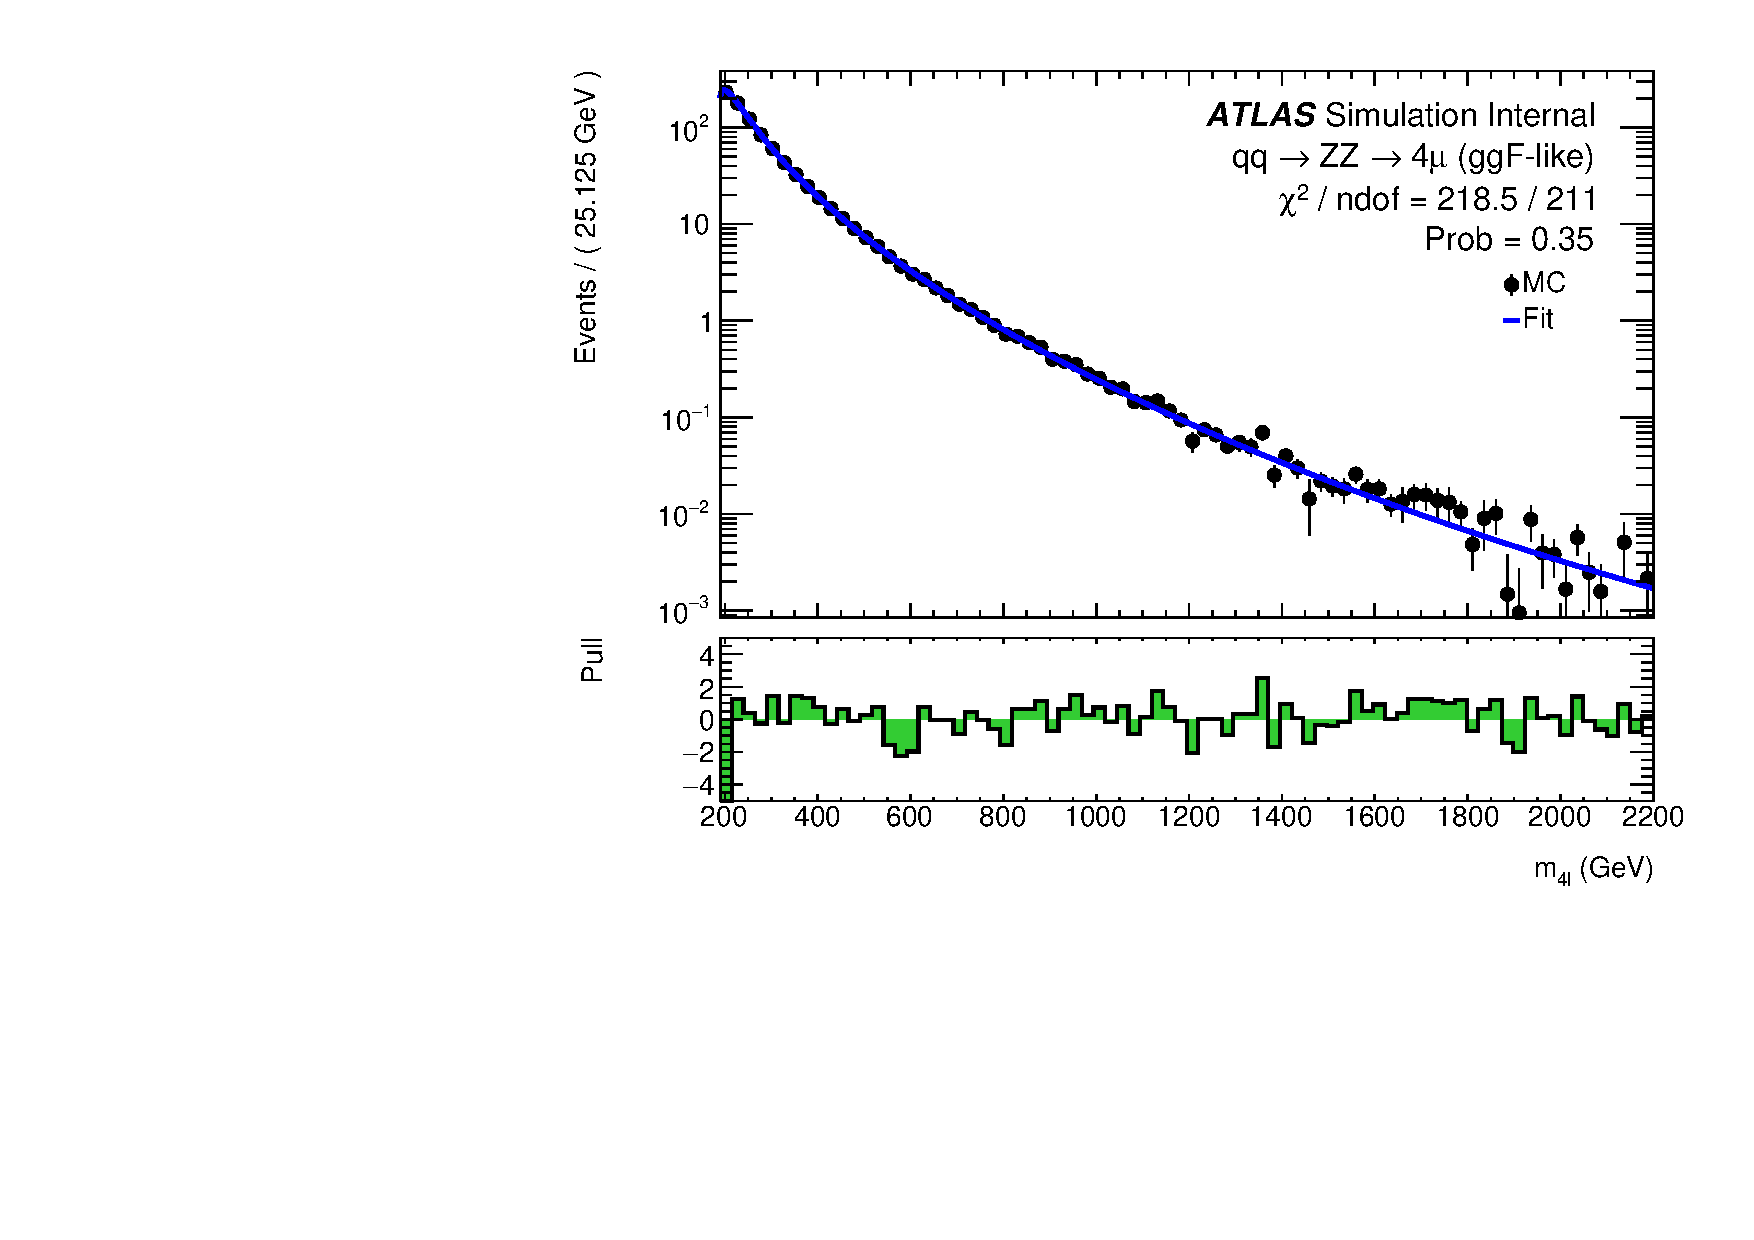
\includegraphics[width=0.32\textwidth]{figures/HMHZZ/background/cut_based/bkg_shape_qqZZ_ggF_4mu_190_to_2200_log.pdf}
    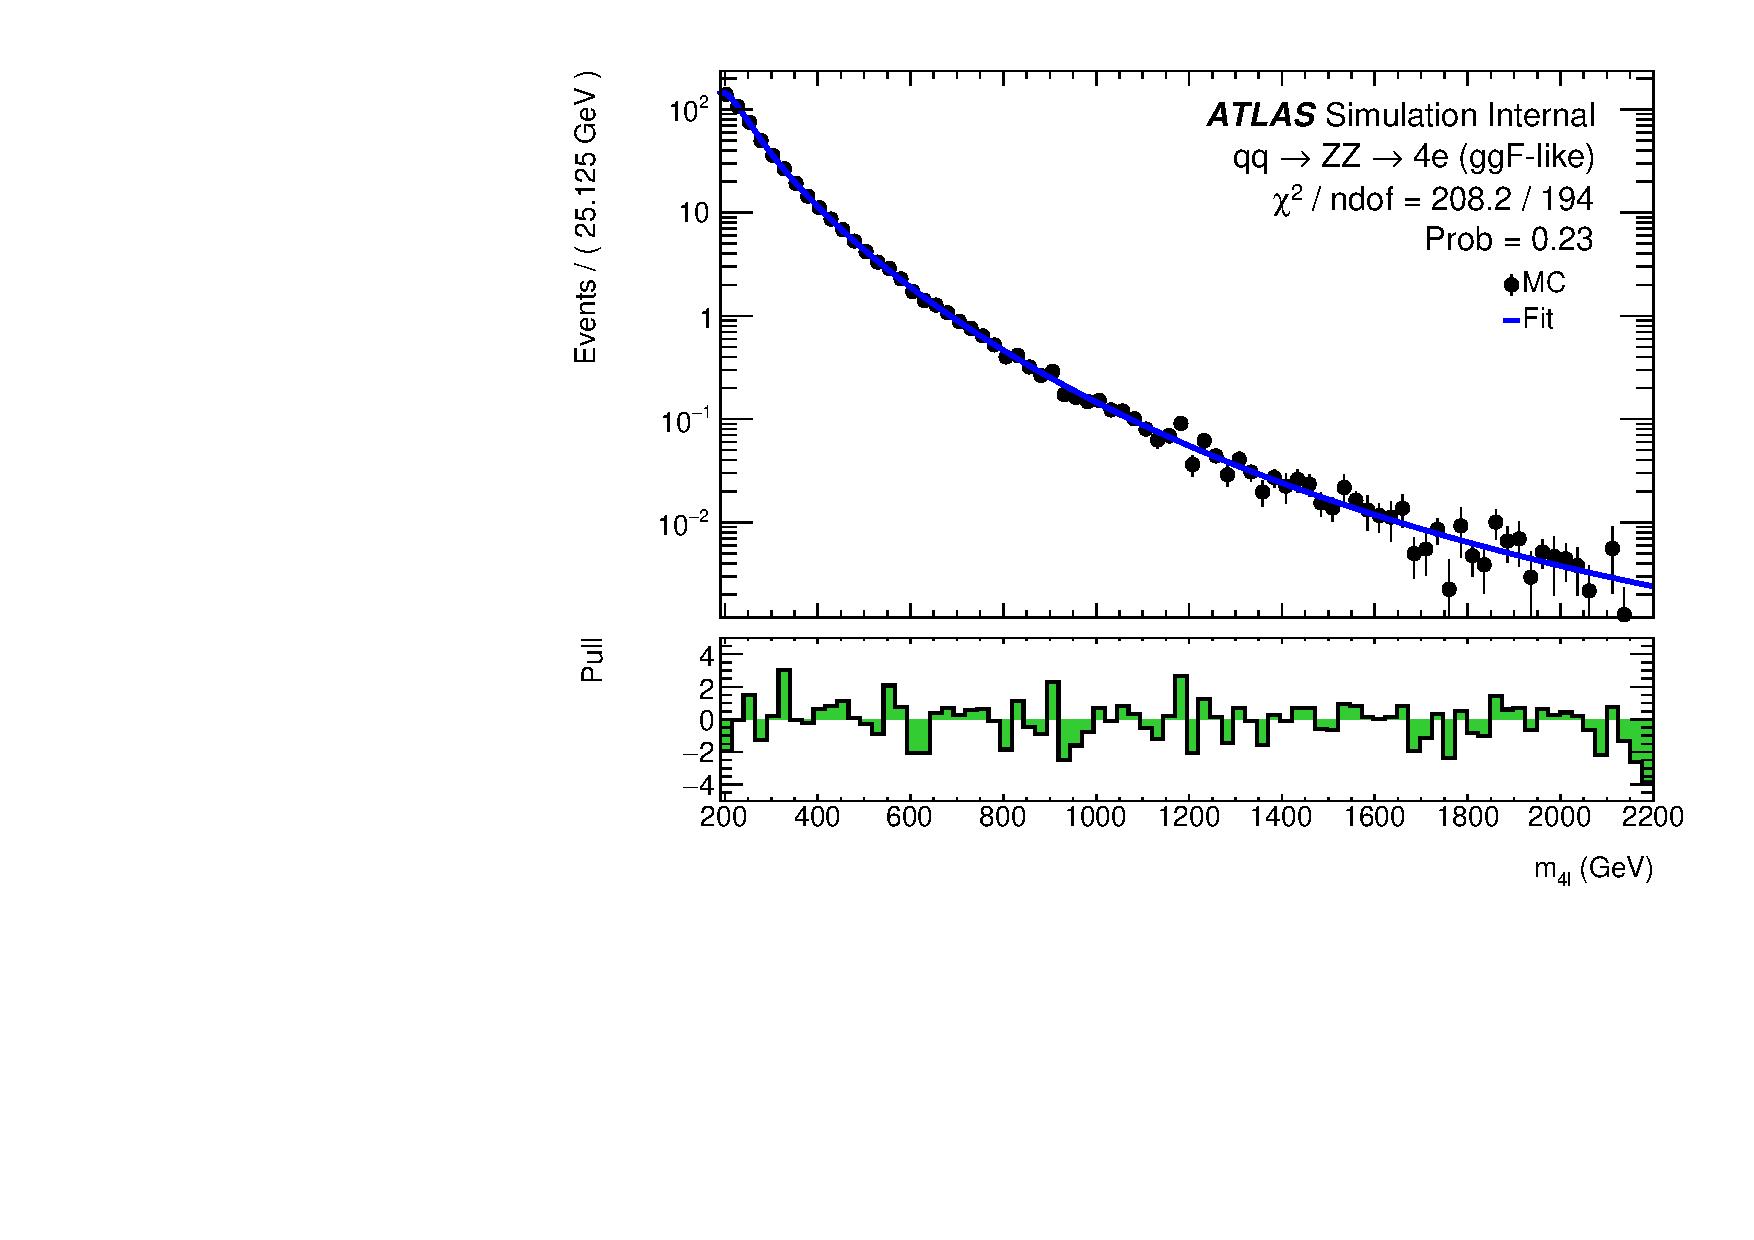
\includegraphics[width=0.32\textwidth]{figures/HMHZZ/background/cut_based/bkg_shape_qqZZ_ggF_4e_190_to_2200_log.pdf} \\
    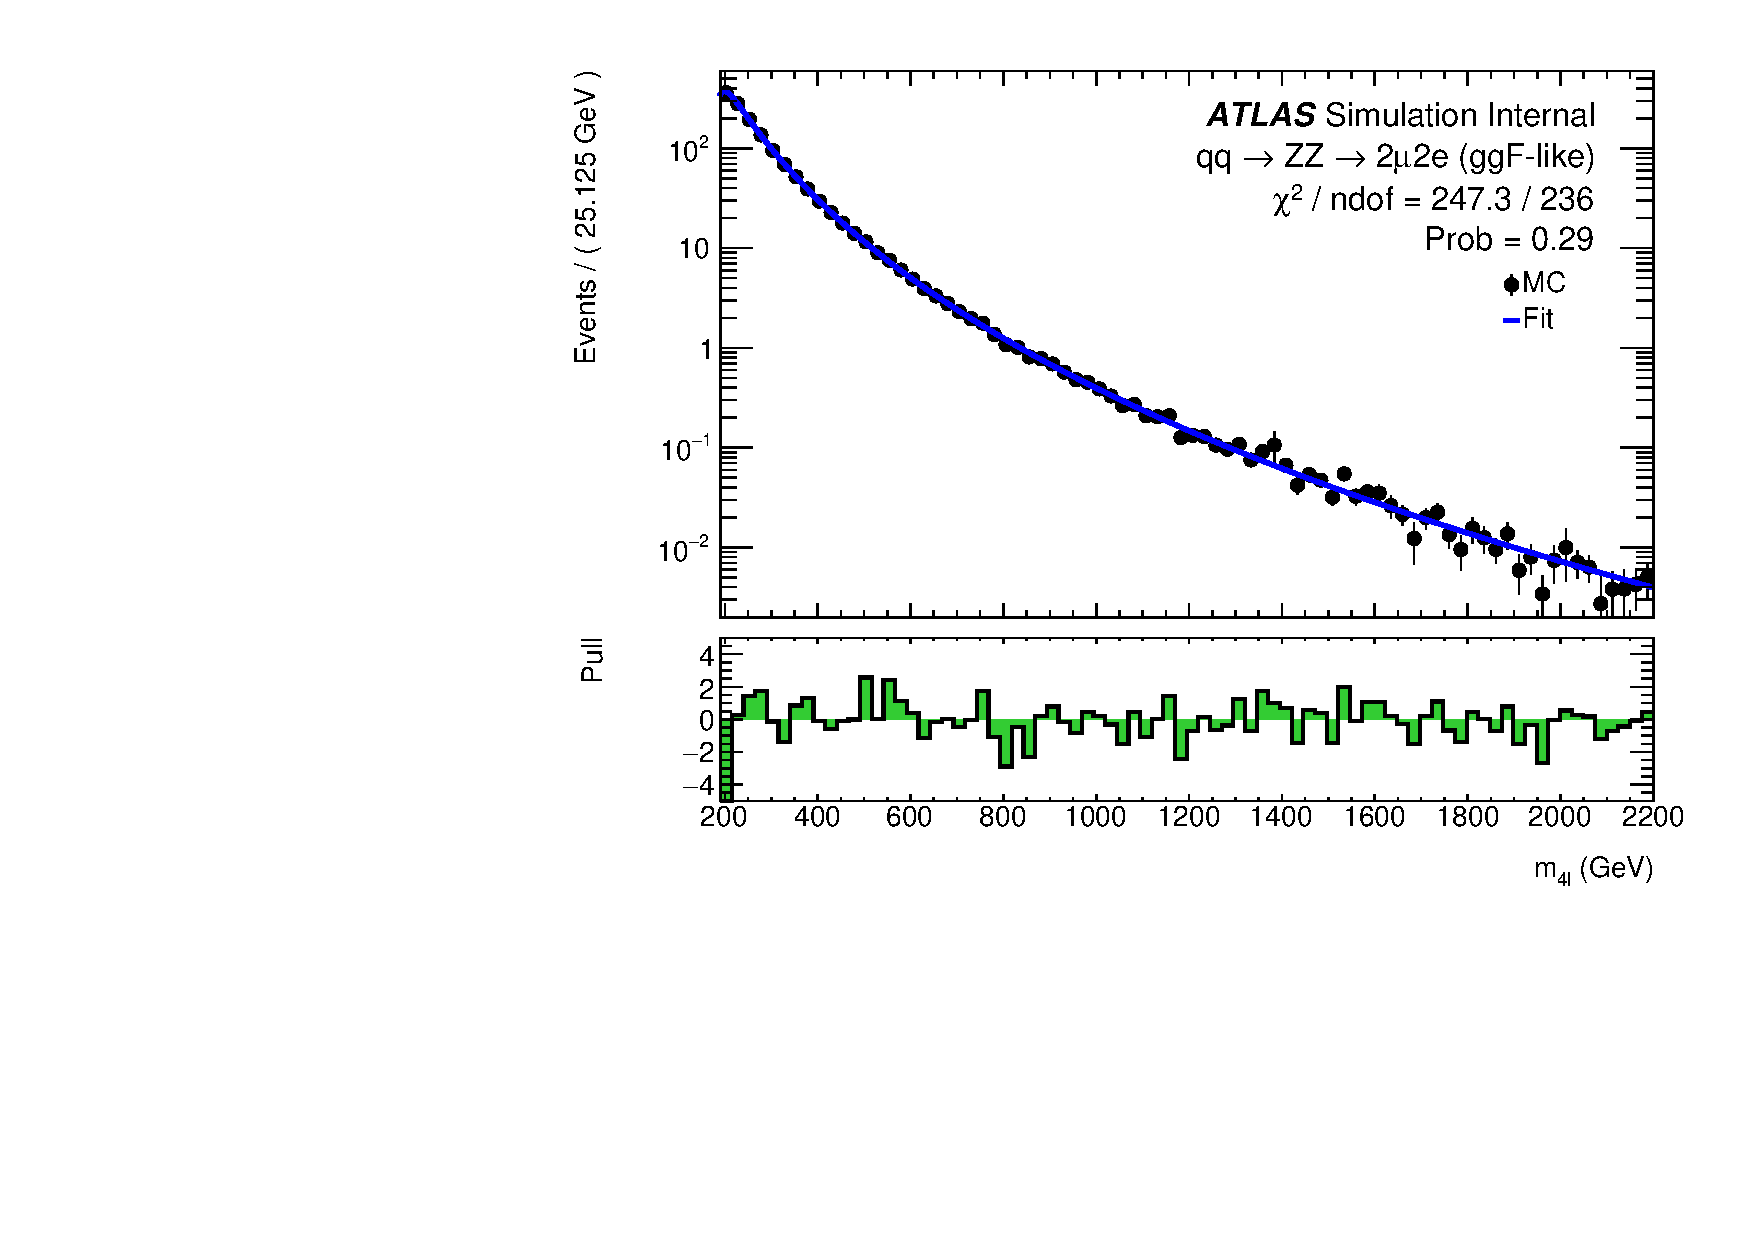
\includegraphics[width=0.32\textwidth]{figures/HMHZZ/background/cut_based/bkg_shape_qqZZ_ggF_2mu2e_190_to_2200_log.pdf}
    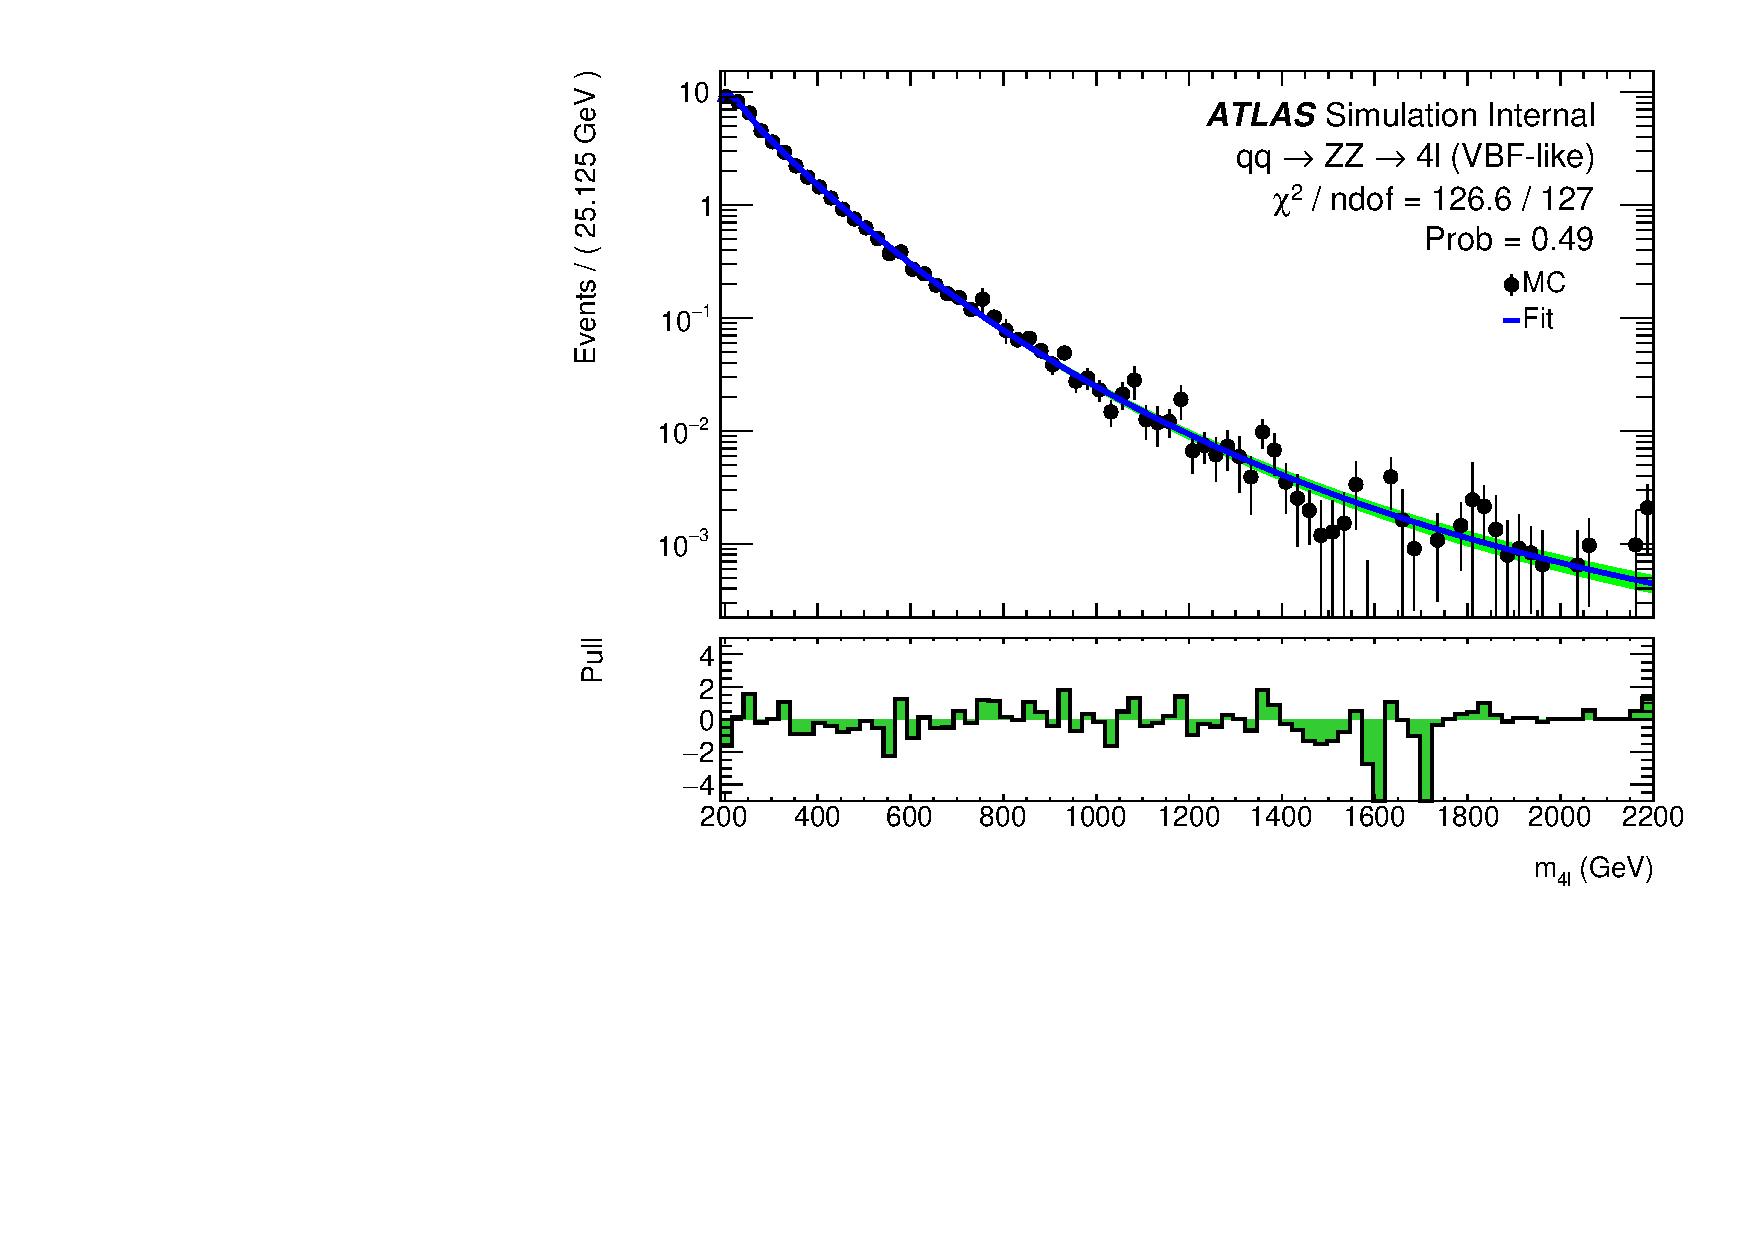
\includegraphics[width=0.32\textwidth]{figures/HMHZZ/background/cut_based/bkg_shape_qqZZ_VBF_incl_190_to_2200_log.pdf}
    \caption{Distributions of the \mfl invariant mass fit projections of the \qqZZ background samples for the $4\mu$,
    $4e$ and $2\mu 2e$ final states in the ggF-CBA-enriched category, and the $4\ell$ inclusive VBF-CBA-enriched category.
    Cut-based categorization is used.} 
    \label{fig:qqZZ_m4l_shape_all_cut_based}
\end{figure}

\begin{figure}[htbp]
    \centering
    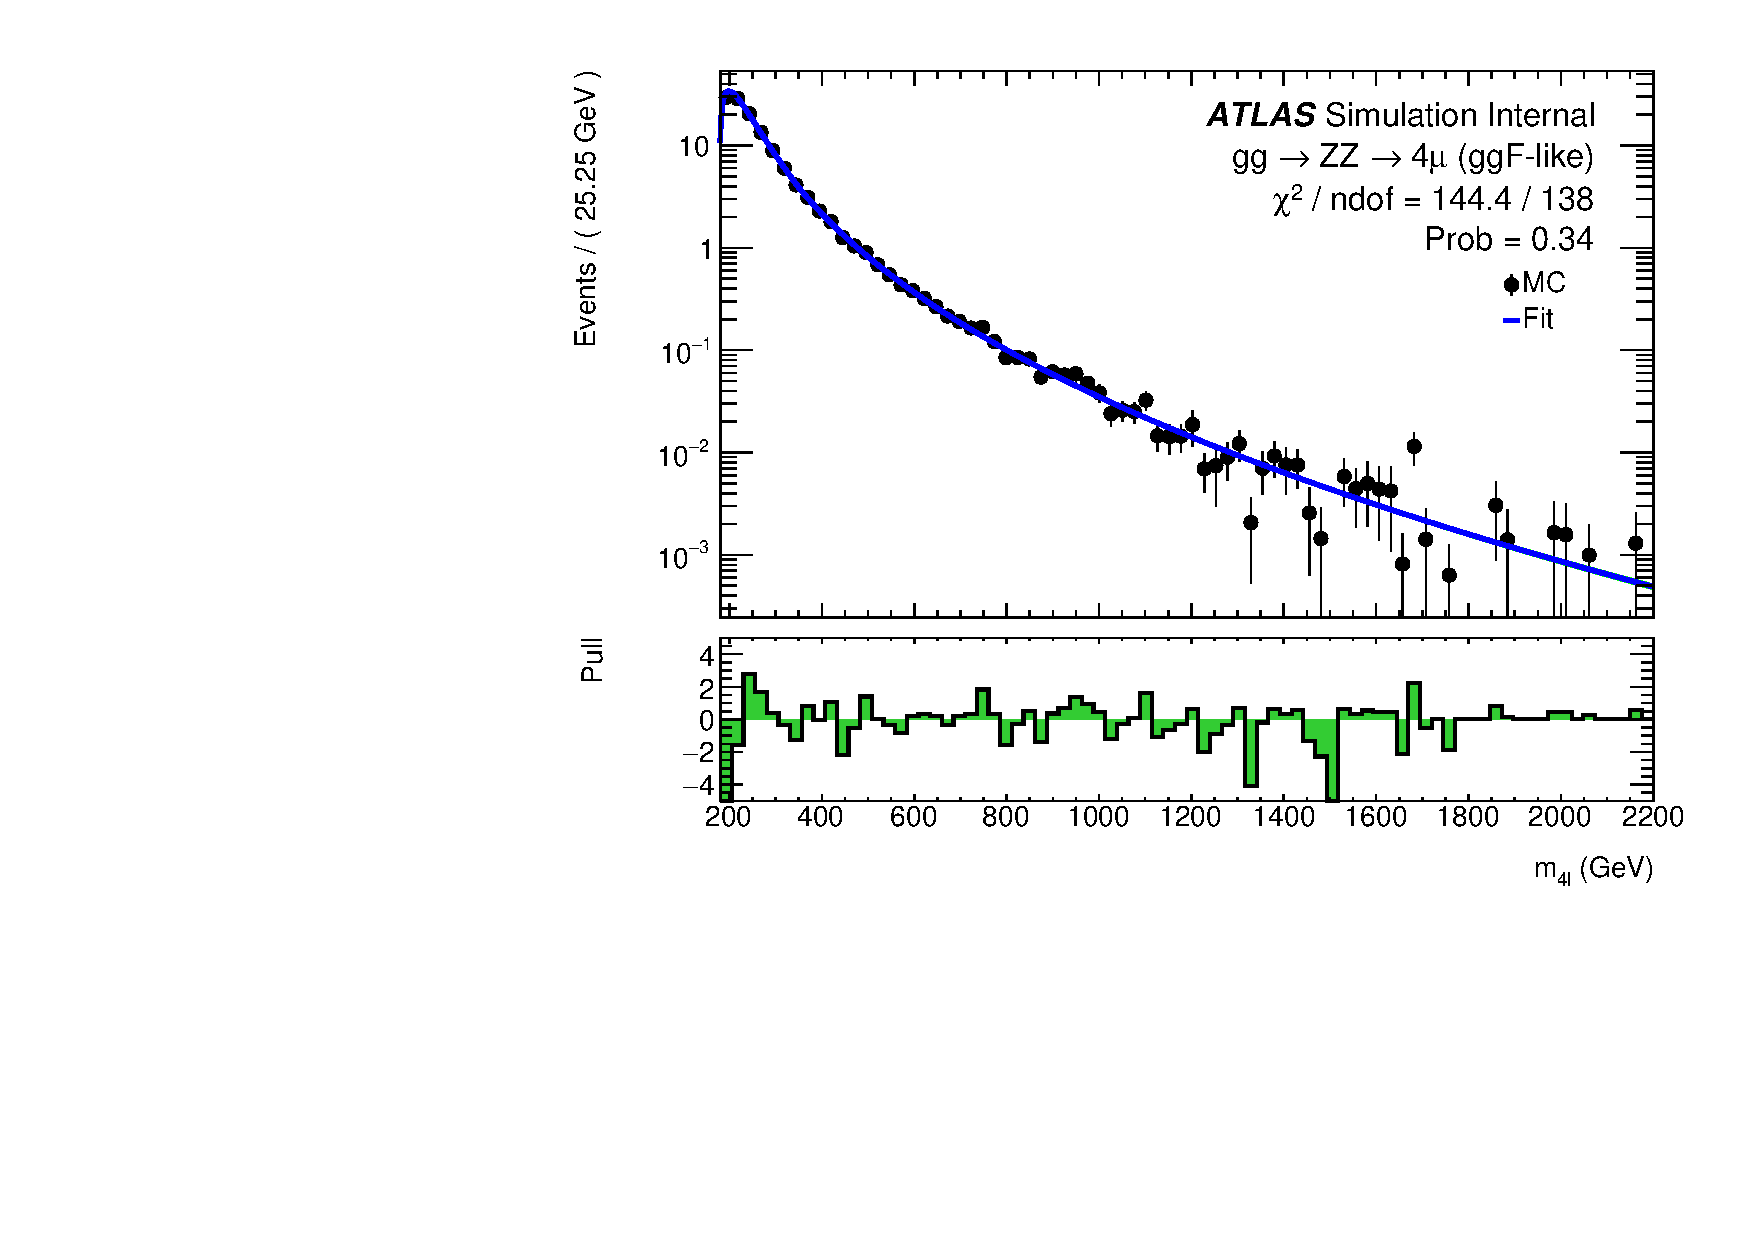
\includegraphics[width=0.32\textwidth]{figures/HMHZZ/background/cut_based/bkg_shape_ggZZ_ggF_4mu_180_to_2200_log.pdf}
    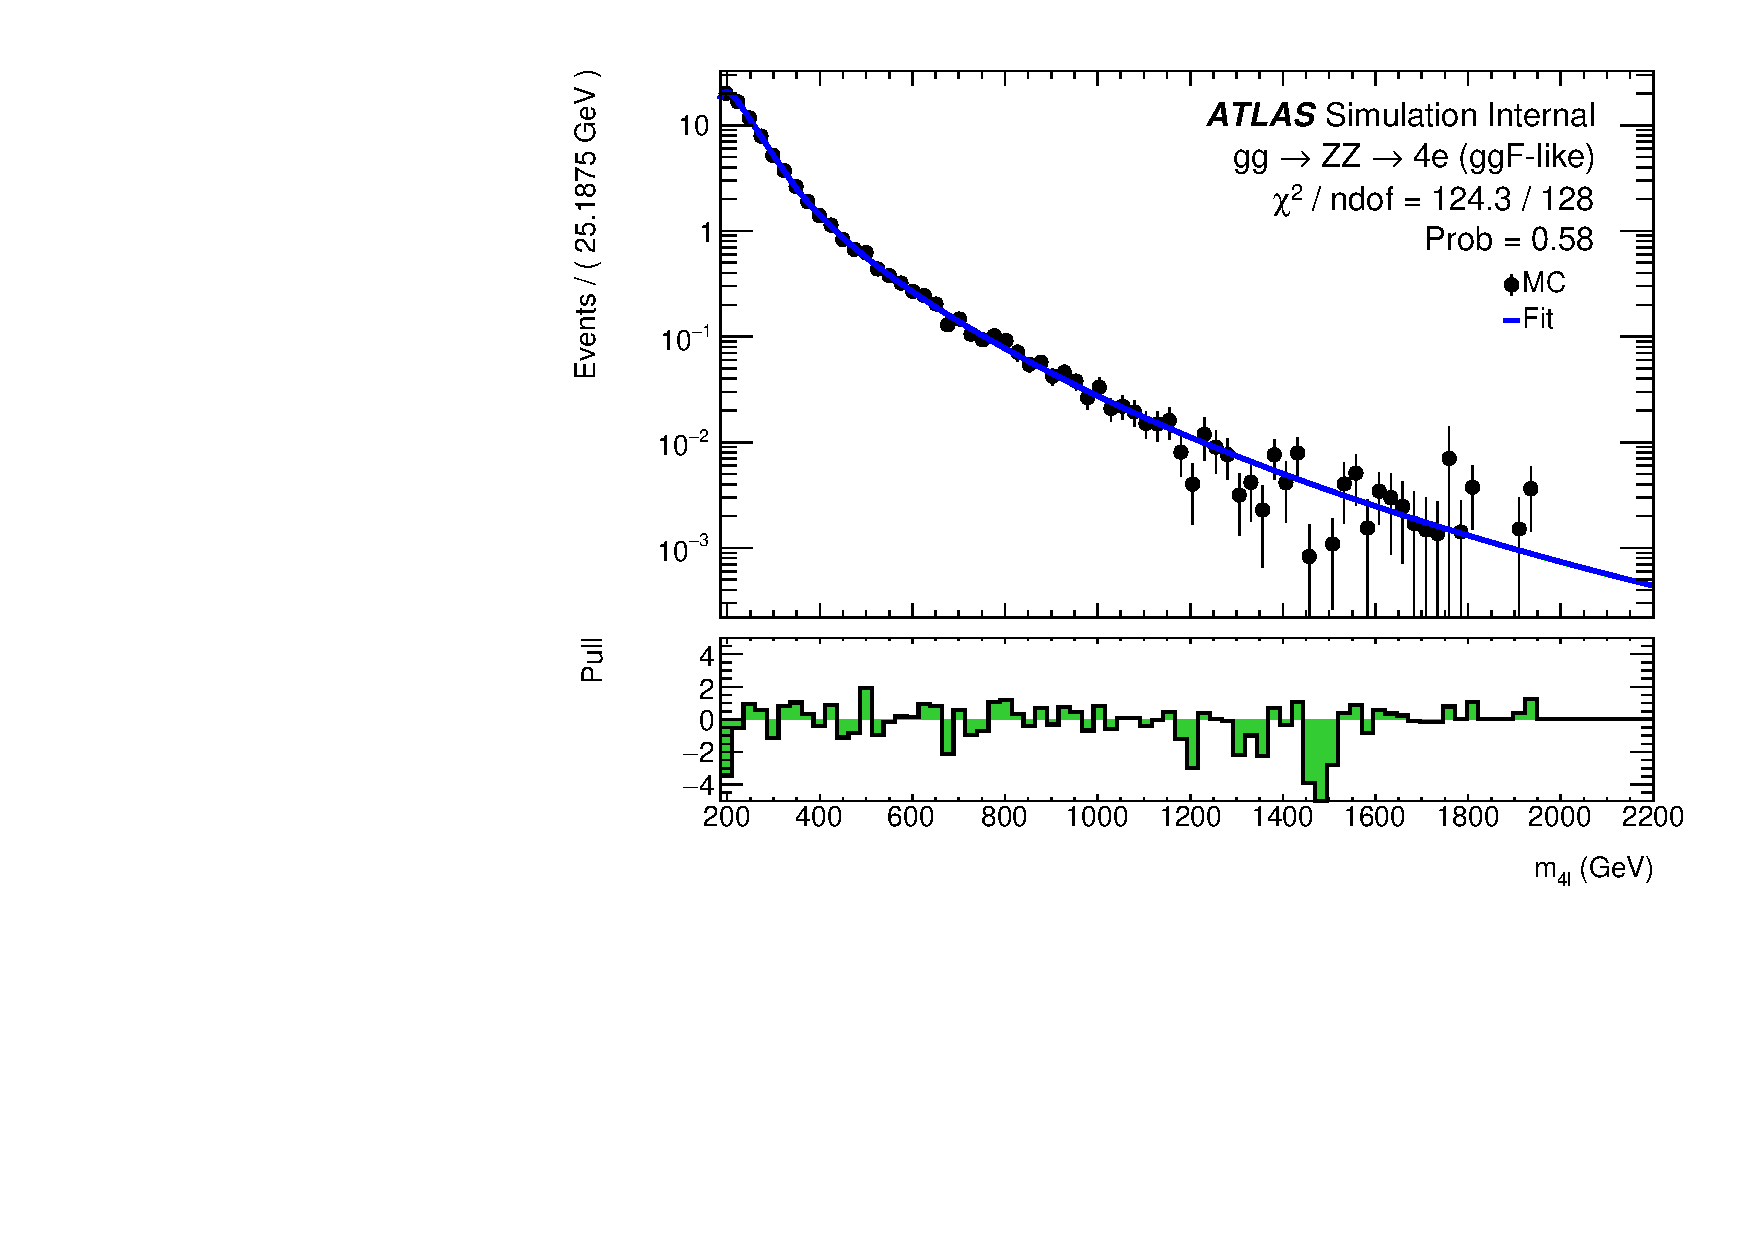
\includegraphics[width=0.32\textwidth]{figures/HMHZZ/background/cut_based/bkg_shape_ggZZ_ggF_4e_185_to_2200_log.pdf} \\
    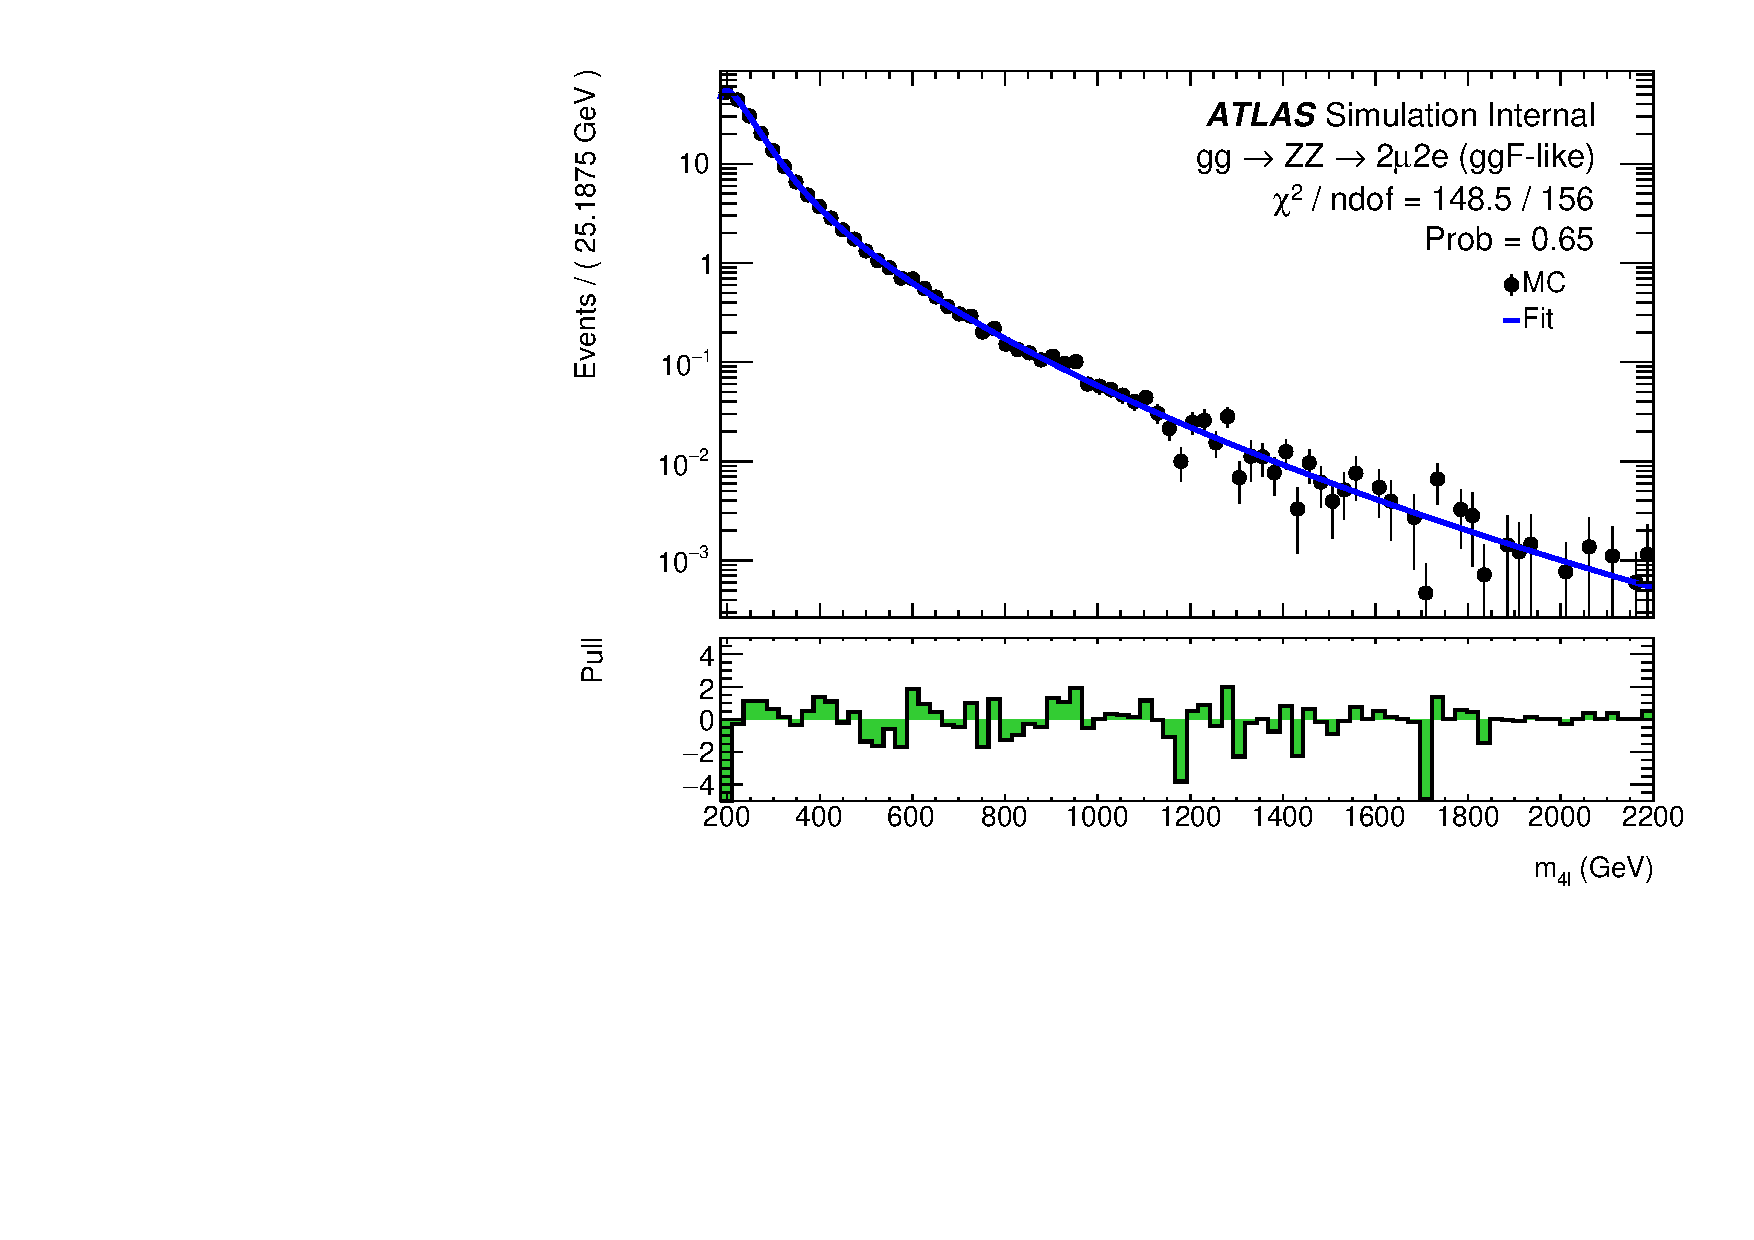
\includegraphics[width=0.32\textwidth]{figures/HMHZZ/background/cut_based/bkg_shape_ggZZ_ggF_2mu2e_185_to_2200_log.pdf}
    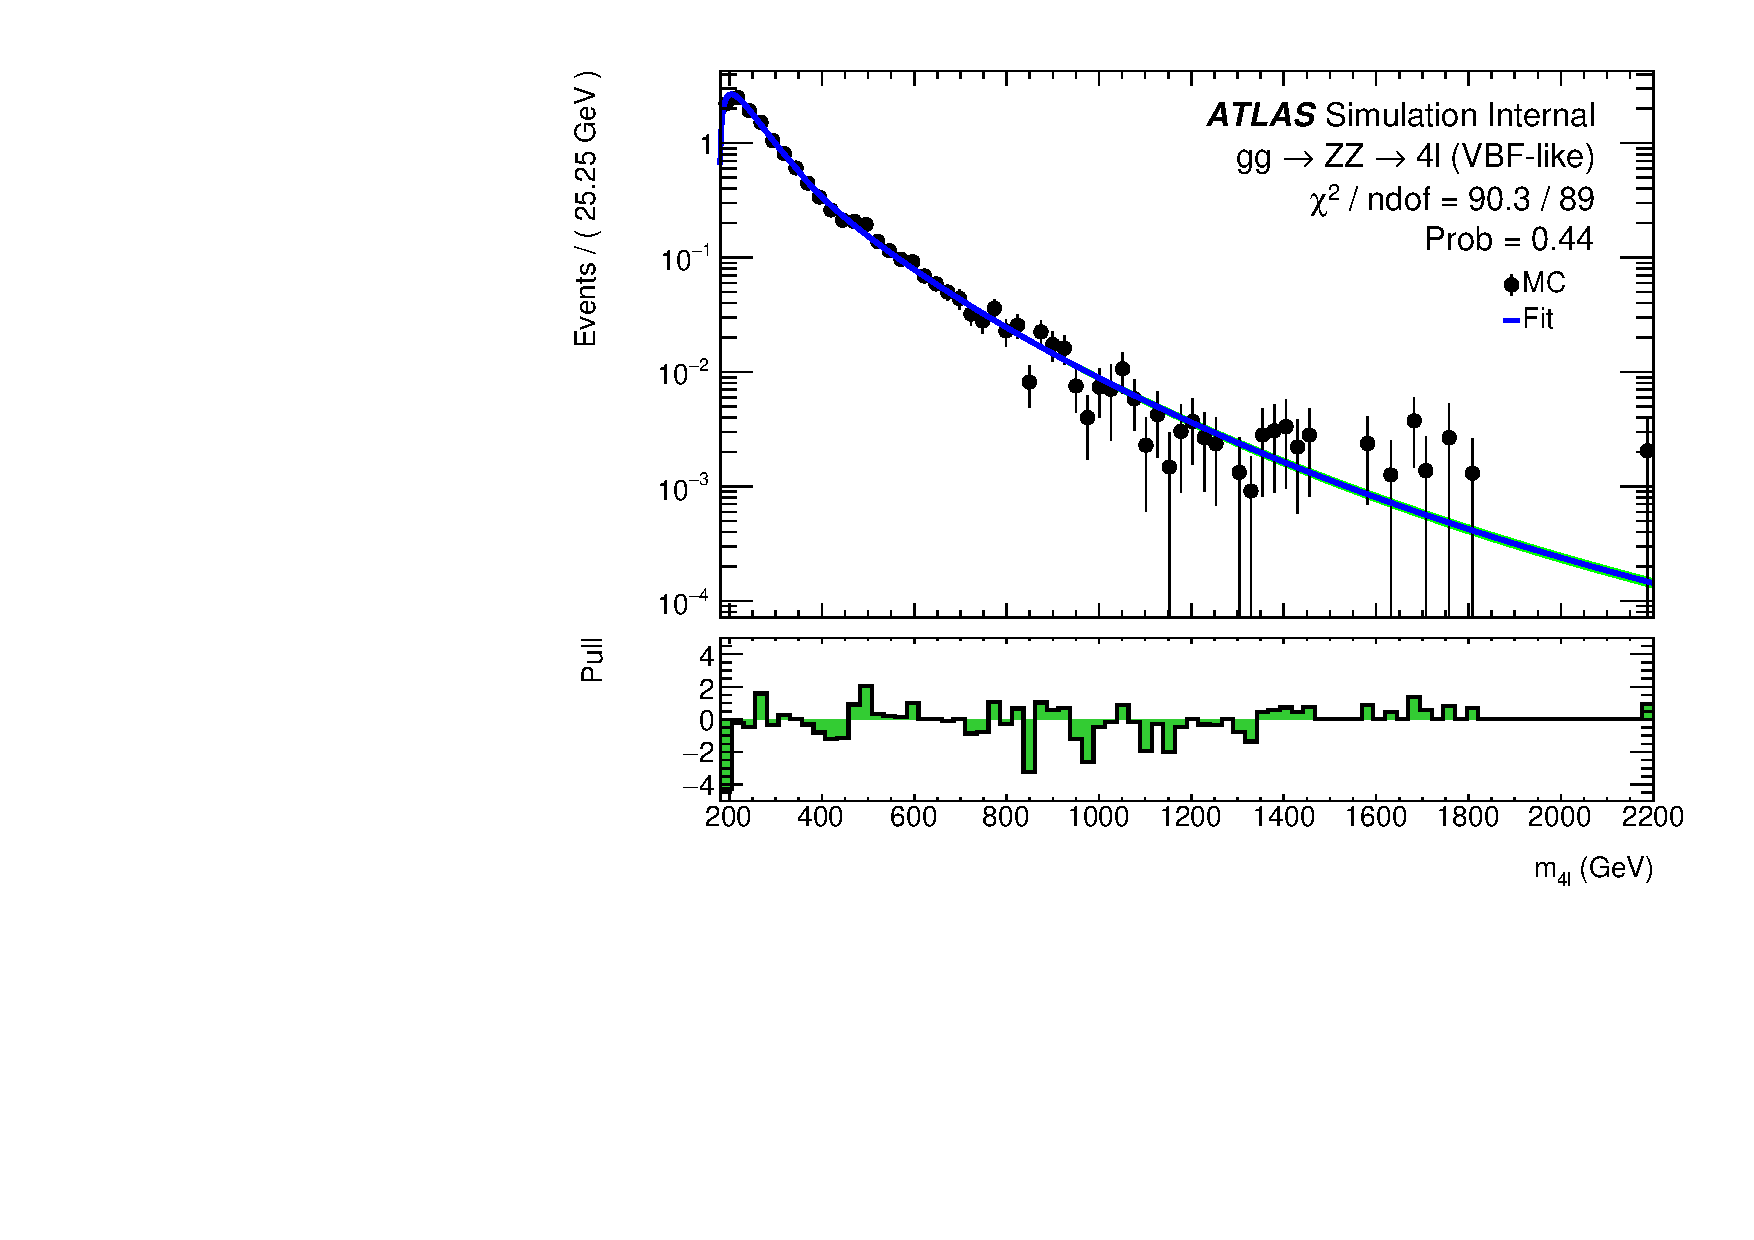
\includegraphics[width=0.32\textwidth]{figures/HMHZZ/background/cut_based/bkg_shape_ggZZ_VBF_incl_180_to_2200_log.pdf}
    \caption{Distributions of the \mfl invariant mass fit projections of the \ggZZ background samples for the $4\mu$,
    $4e$ and $2\mu 2e$ final states in the ggF-CBA-enriched category, and the $4\ell$ inclusive VBF-CBA-enriched category. 
    Cut-based categorization is used.} 
    \label{fig:ggZZ_m4l_shape_all_cut_based}
\end{figure}

\begin{figure}[htbp]
    \centering
    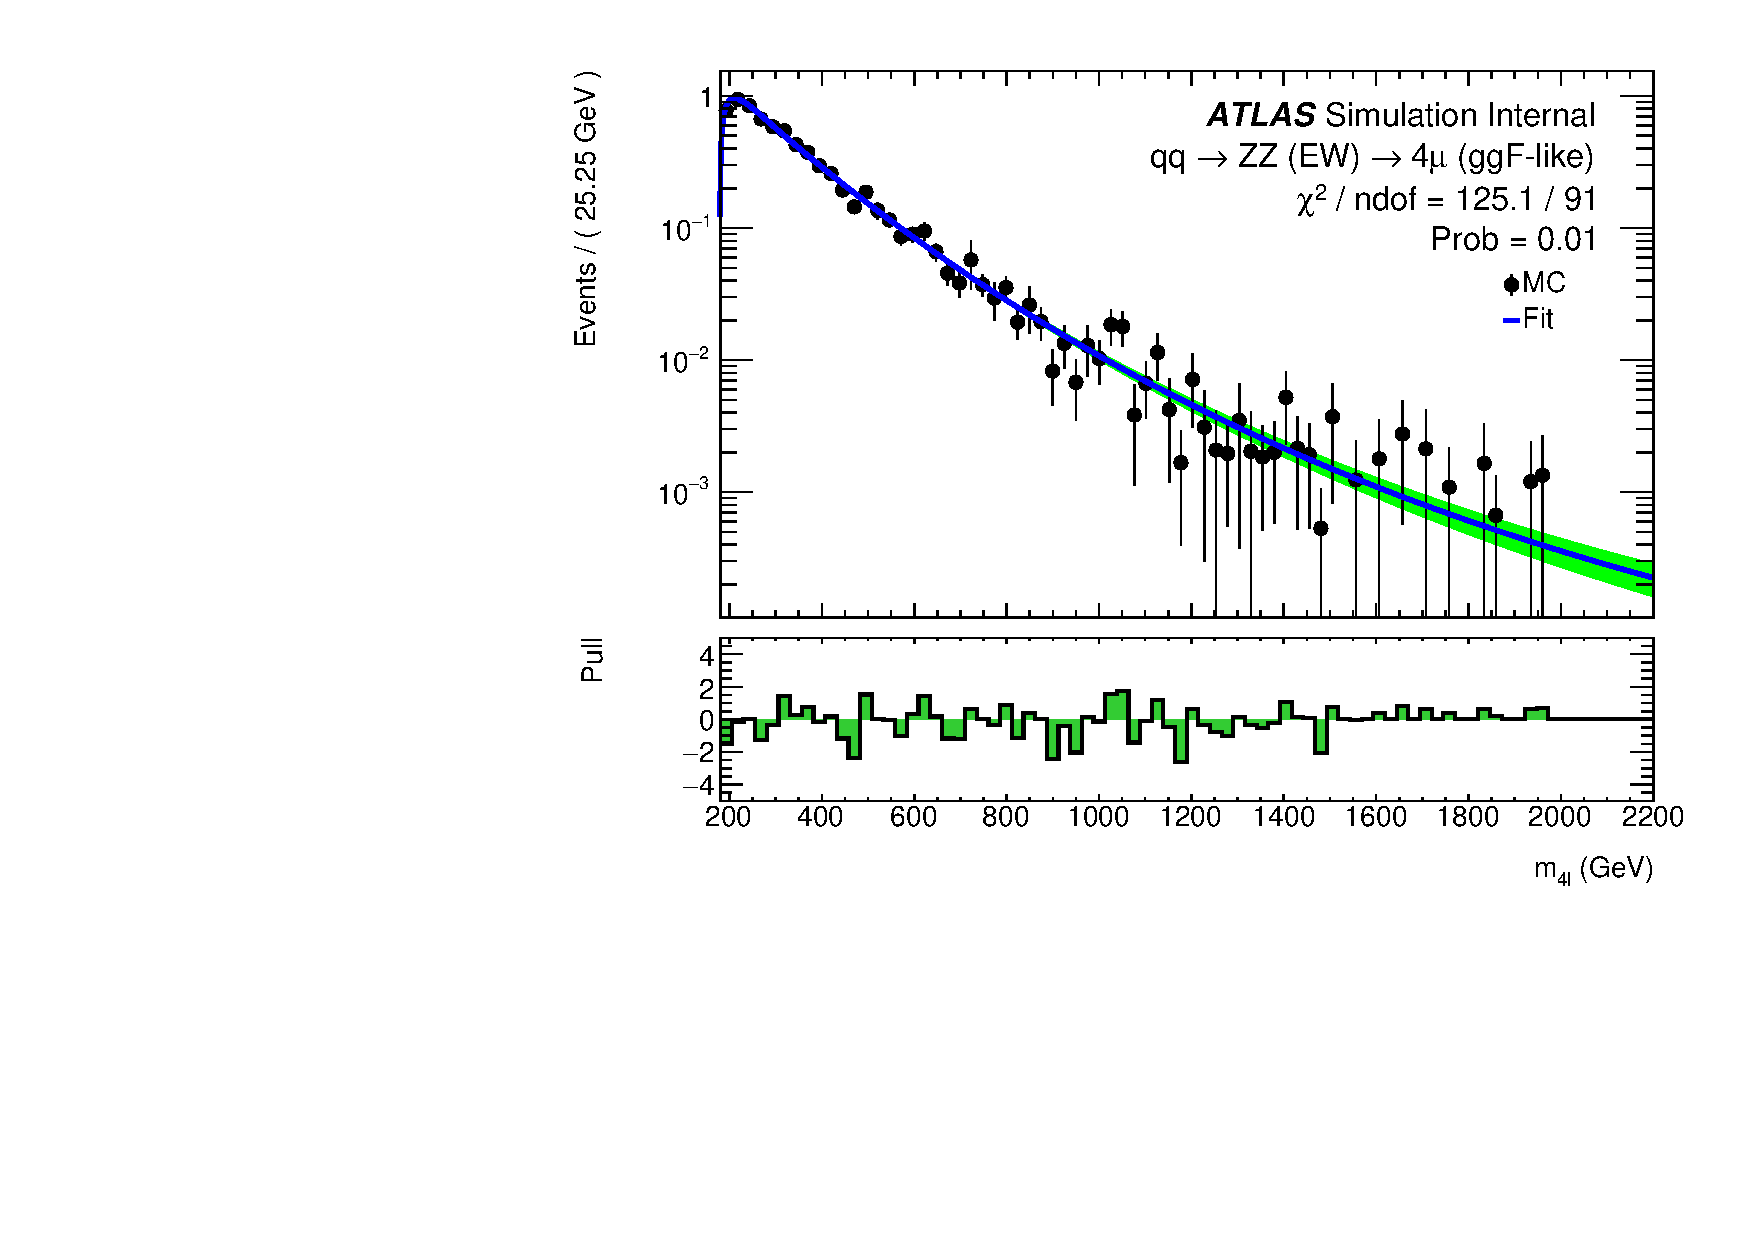
\includegraphics[width=0.32\textwidth]{figures/HMHZZ/background/cut_based/bkg_shape_qqZZEW_ggF_4mu_180_to_2200_log.pdf}
    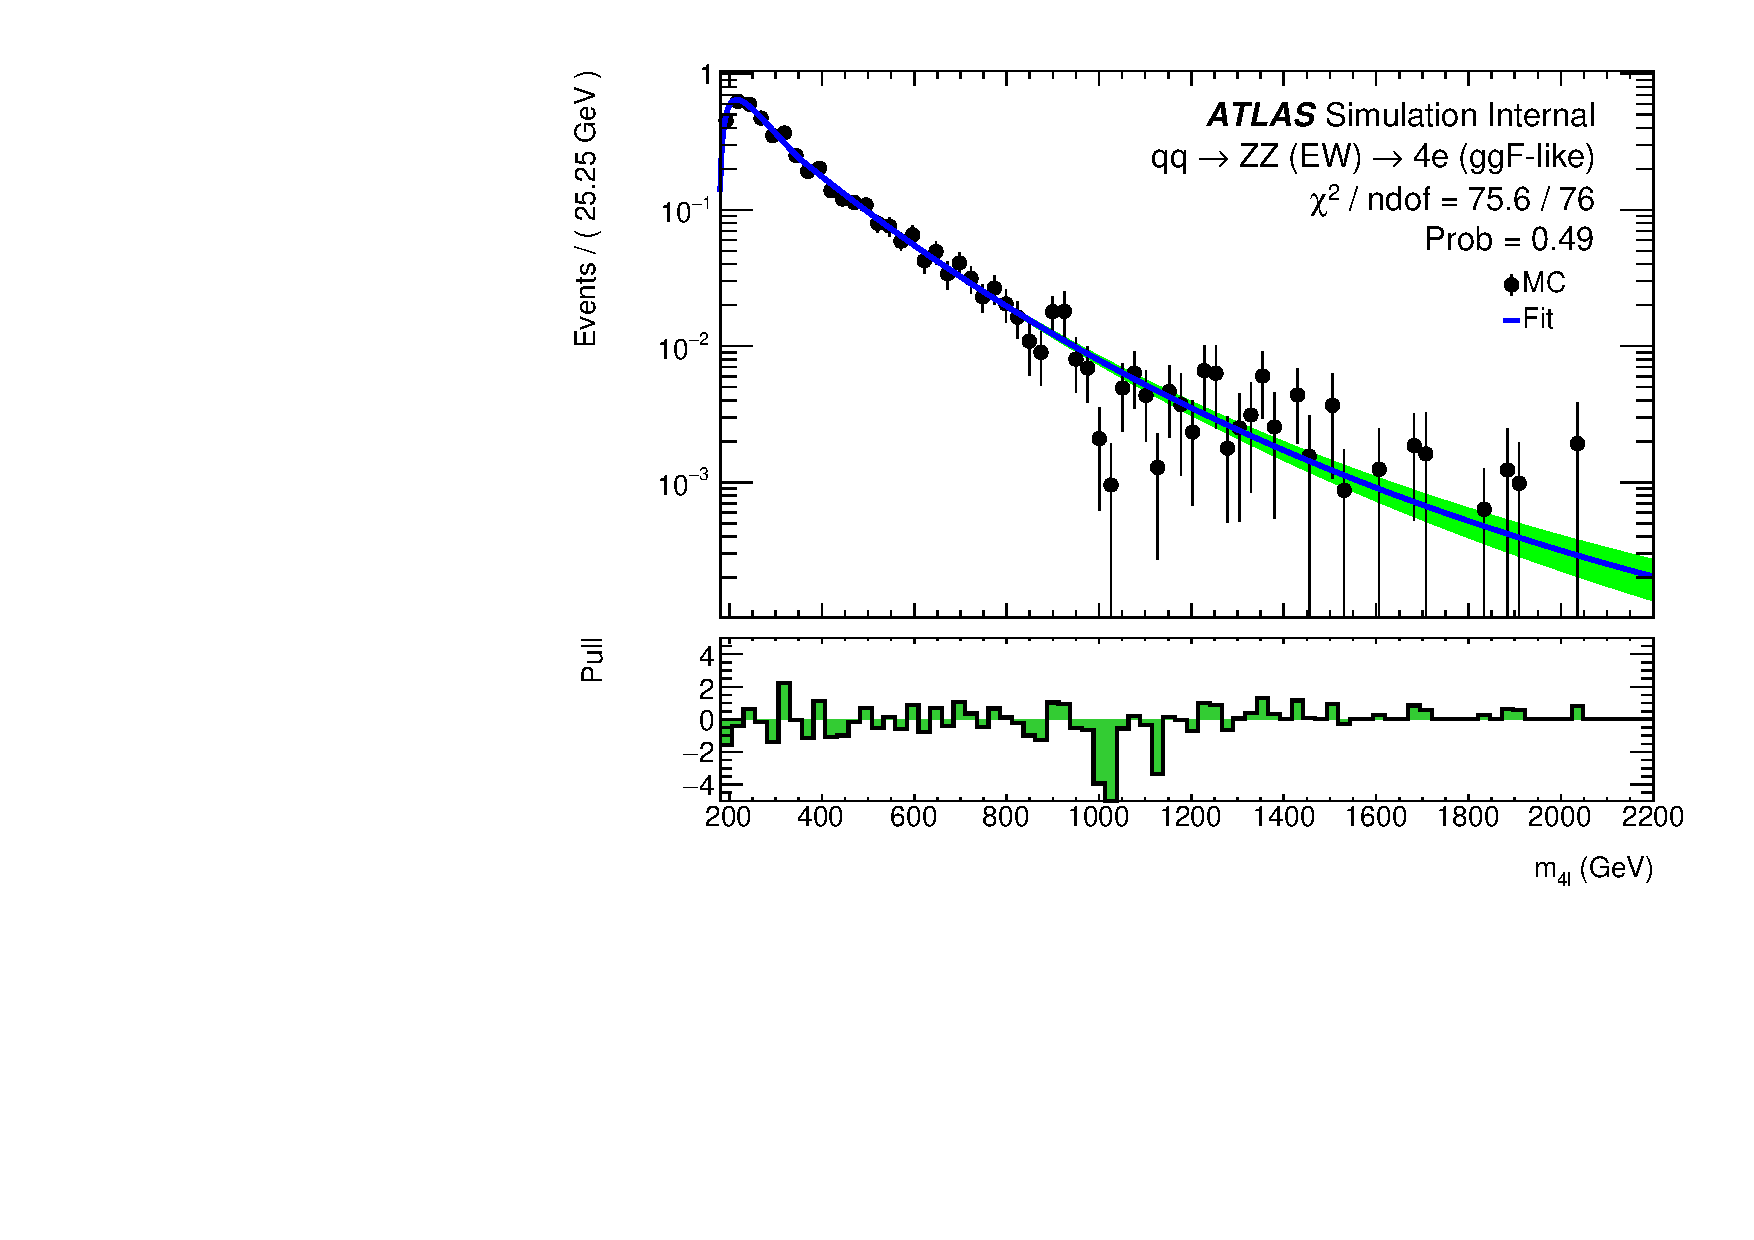
\includegraphics[width=0.32\textwidth]{figures/HMHZZ/background/cut_based/bkg_shape_qqZZEW_ggF_4e_180_to_2200_log.pdf} \\
    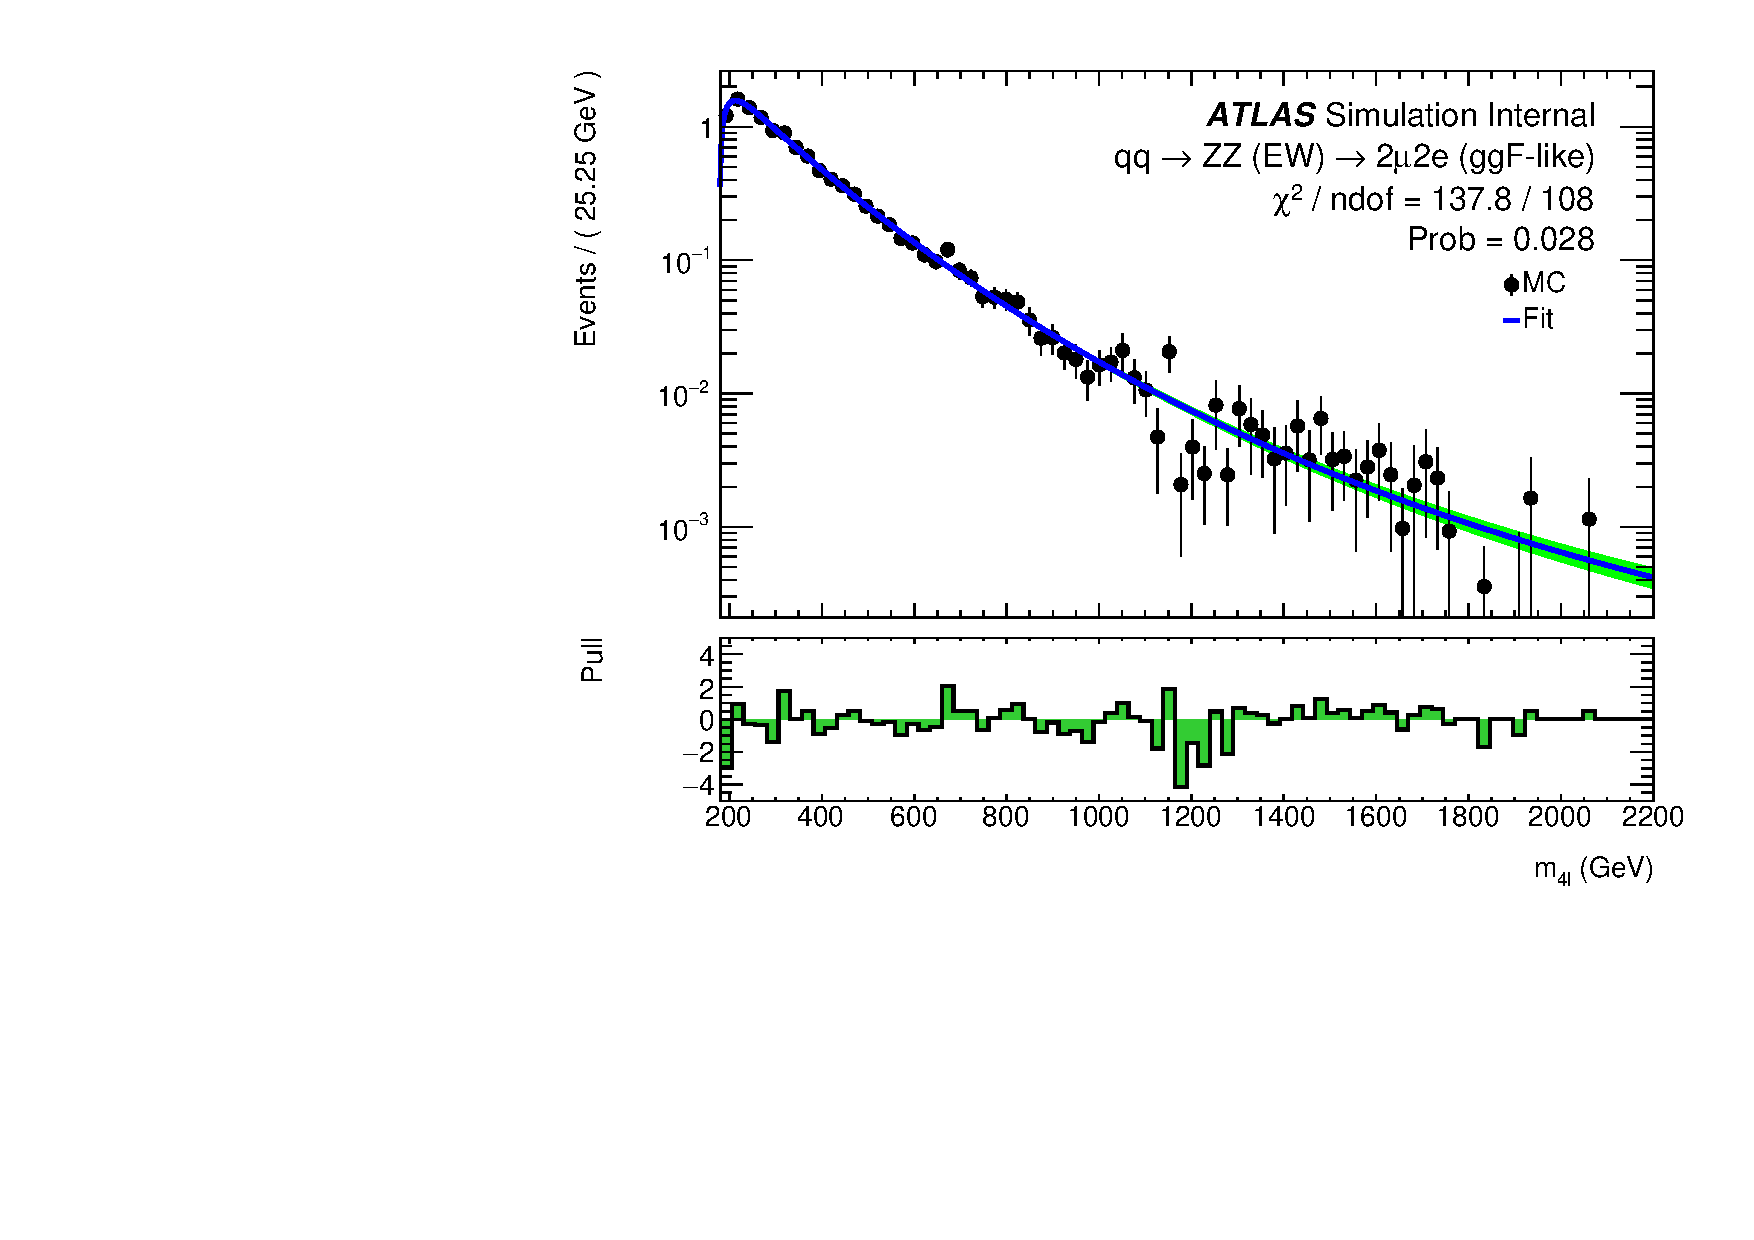
\includegraphics[width=0.32\textwidth]{figures/HMHZZ/background/cut_based/bkg_shape_qqZZEW_ggF_2mu2e_180_to_2200_log.pdf}
    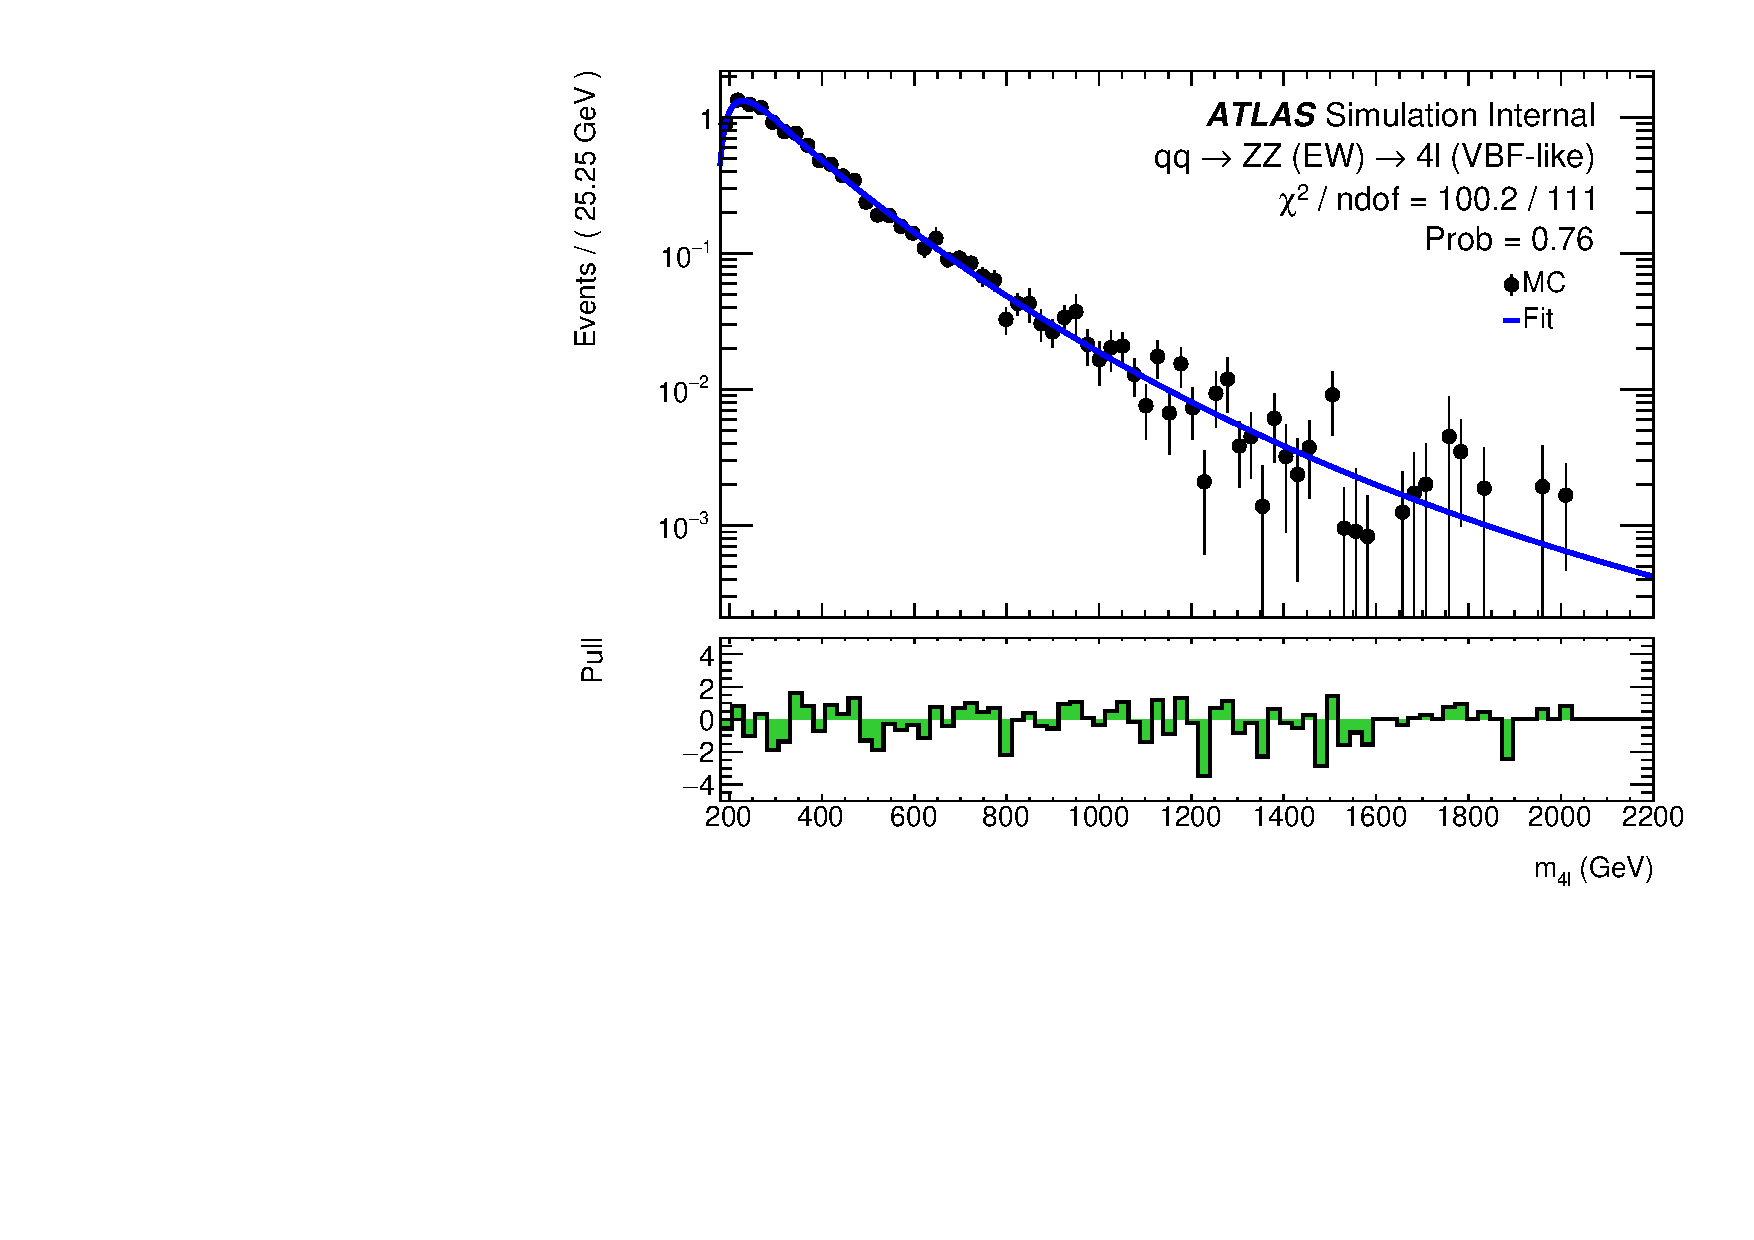
\includegraphics[width=0.32\textwidth]{figures/HMHZZ/background/cut_based/bkg_shape_qqZZEW_VBF_incl_180_to_2200_log.pdf}
    \caption{Distributions of the \mfl invariant mass fit projections of the \qqZZ (EW) background samples for the
    $4\mu$, $4e$ and $2\mu 2e$ final states in the ggF-CBA-enriched category, and the $4\ell$ inclusive VBF-CBA-enriched category. 
    Cut-based categorization is used.} 
    \label{fig:qqZZEW_m4l_shape_all_cut_based}
\end{figure}

%===========================================================================================================================
\begin{figure}[htbp]
    \centering
    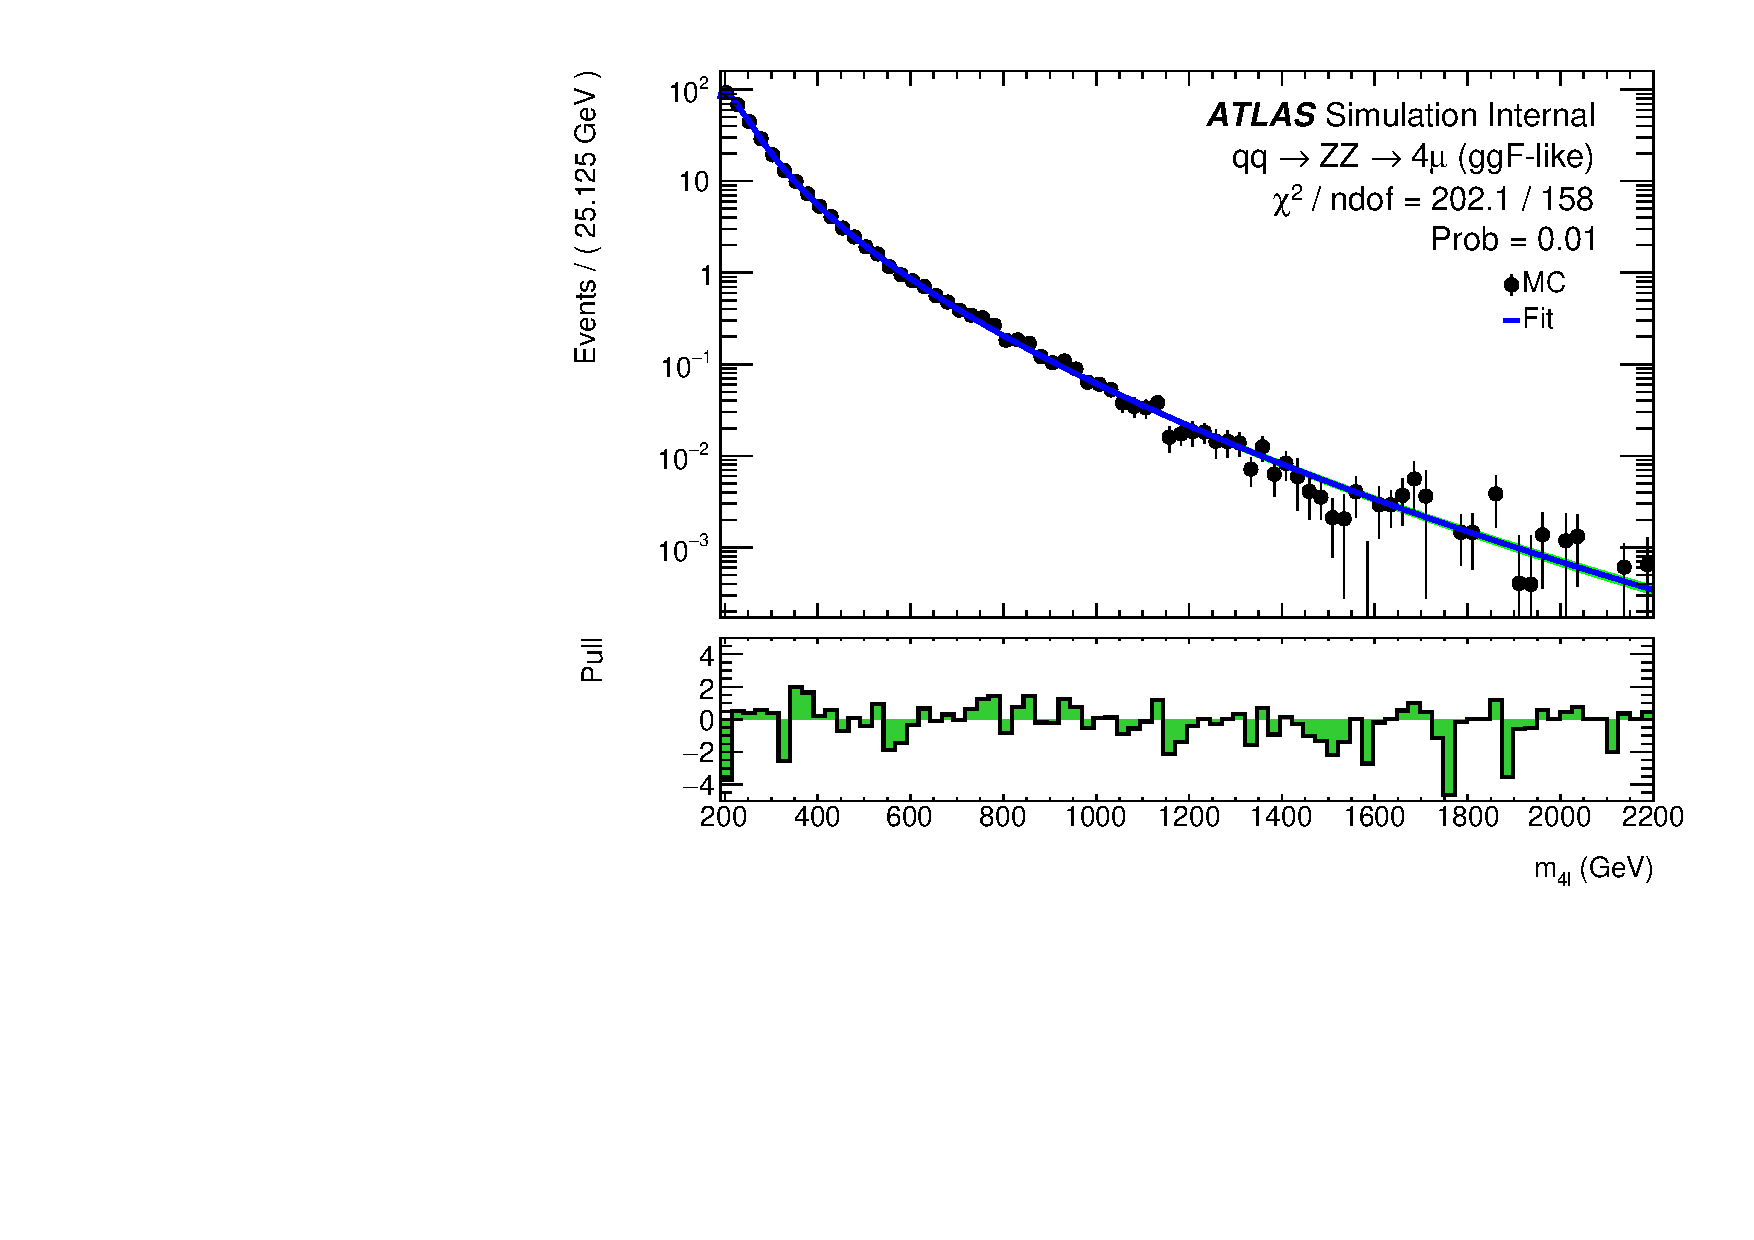
\includegraphics[width=0.32\textwidth]{figures/HMHZZ/background/dnn/bkg_shape_qqZZ_ggF_4mu_190_to_2200_log.pdf}
    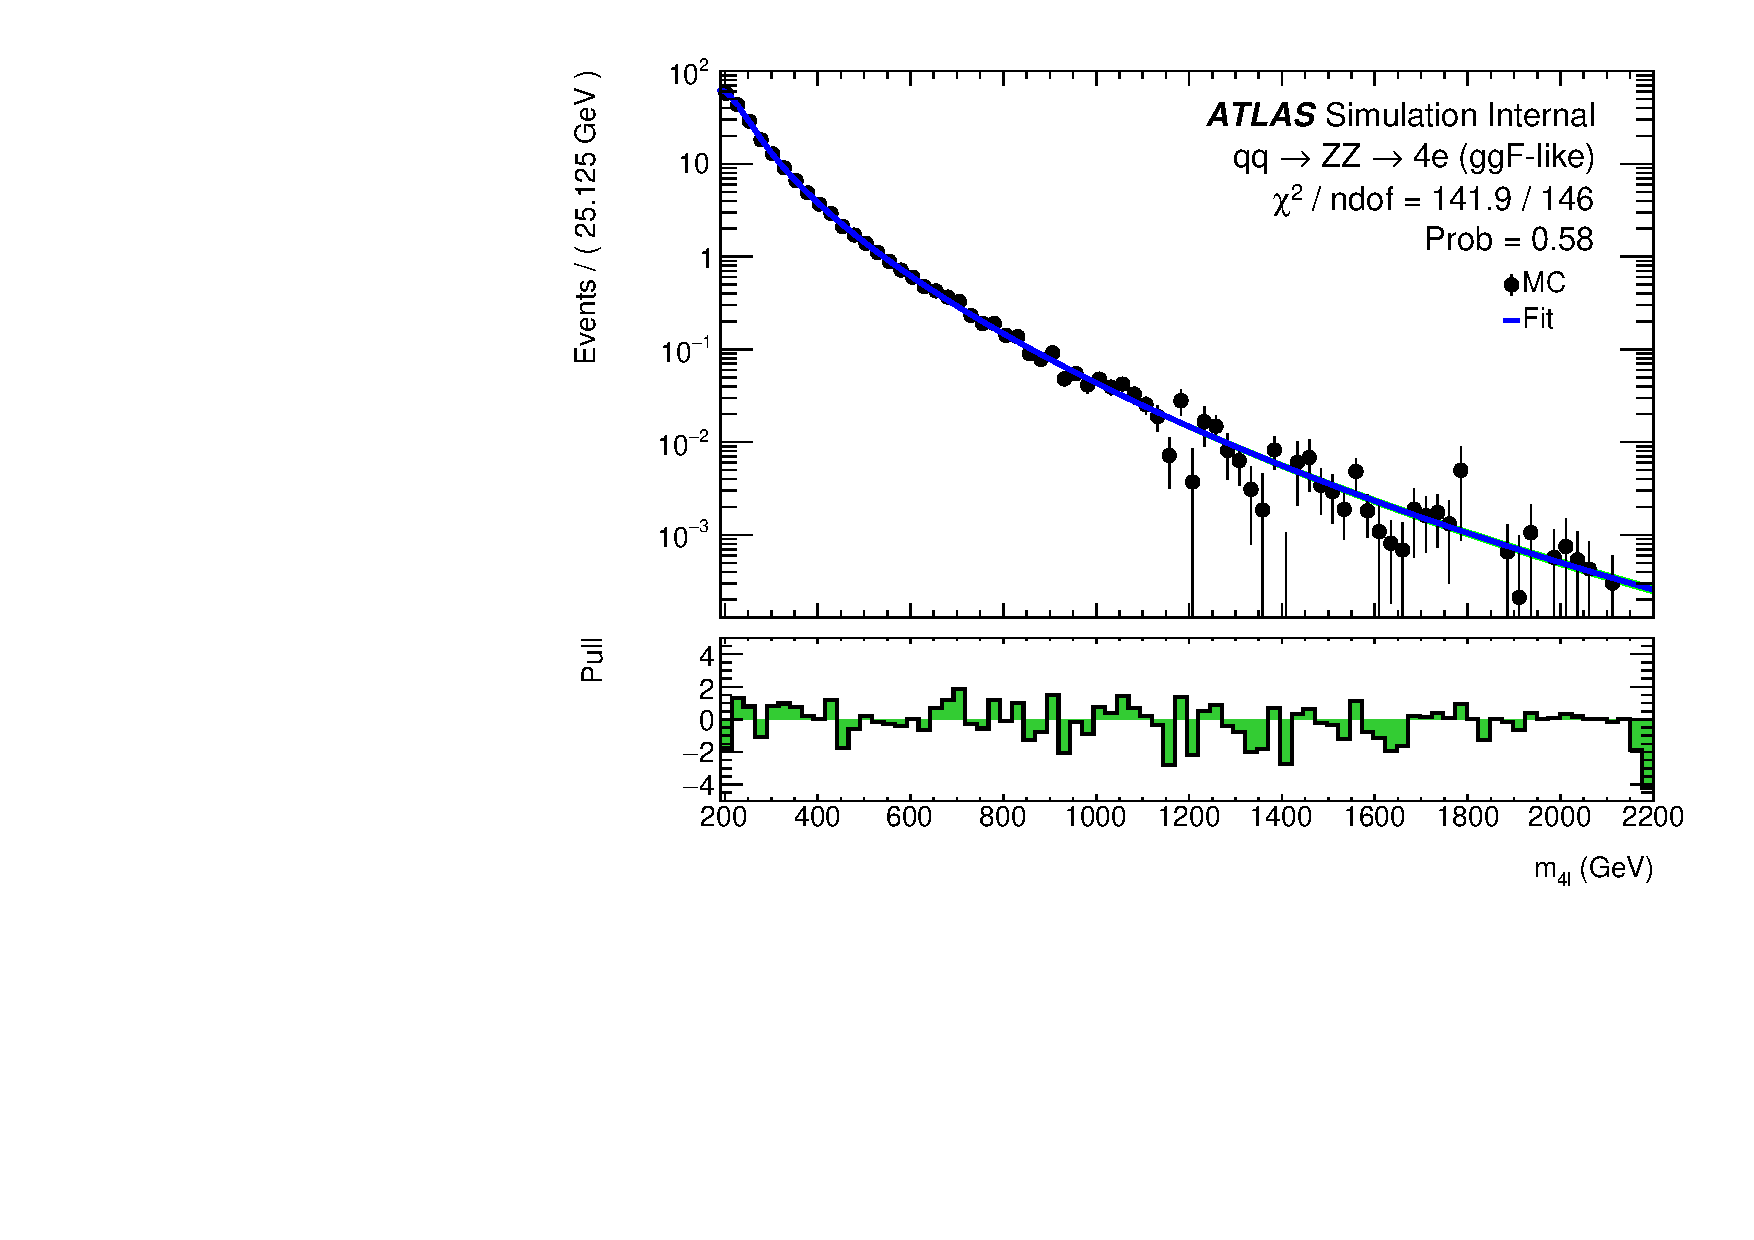
\includegraphics[width=0.32\textwidth]{figures/HMHZZ/background/dnn/bkg_shape_qqZZ_ggF_4e_190_to_2200_log.pdf}
    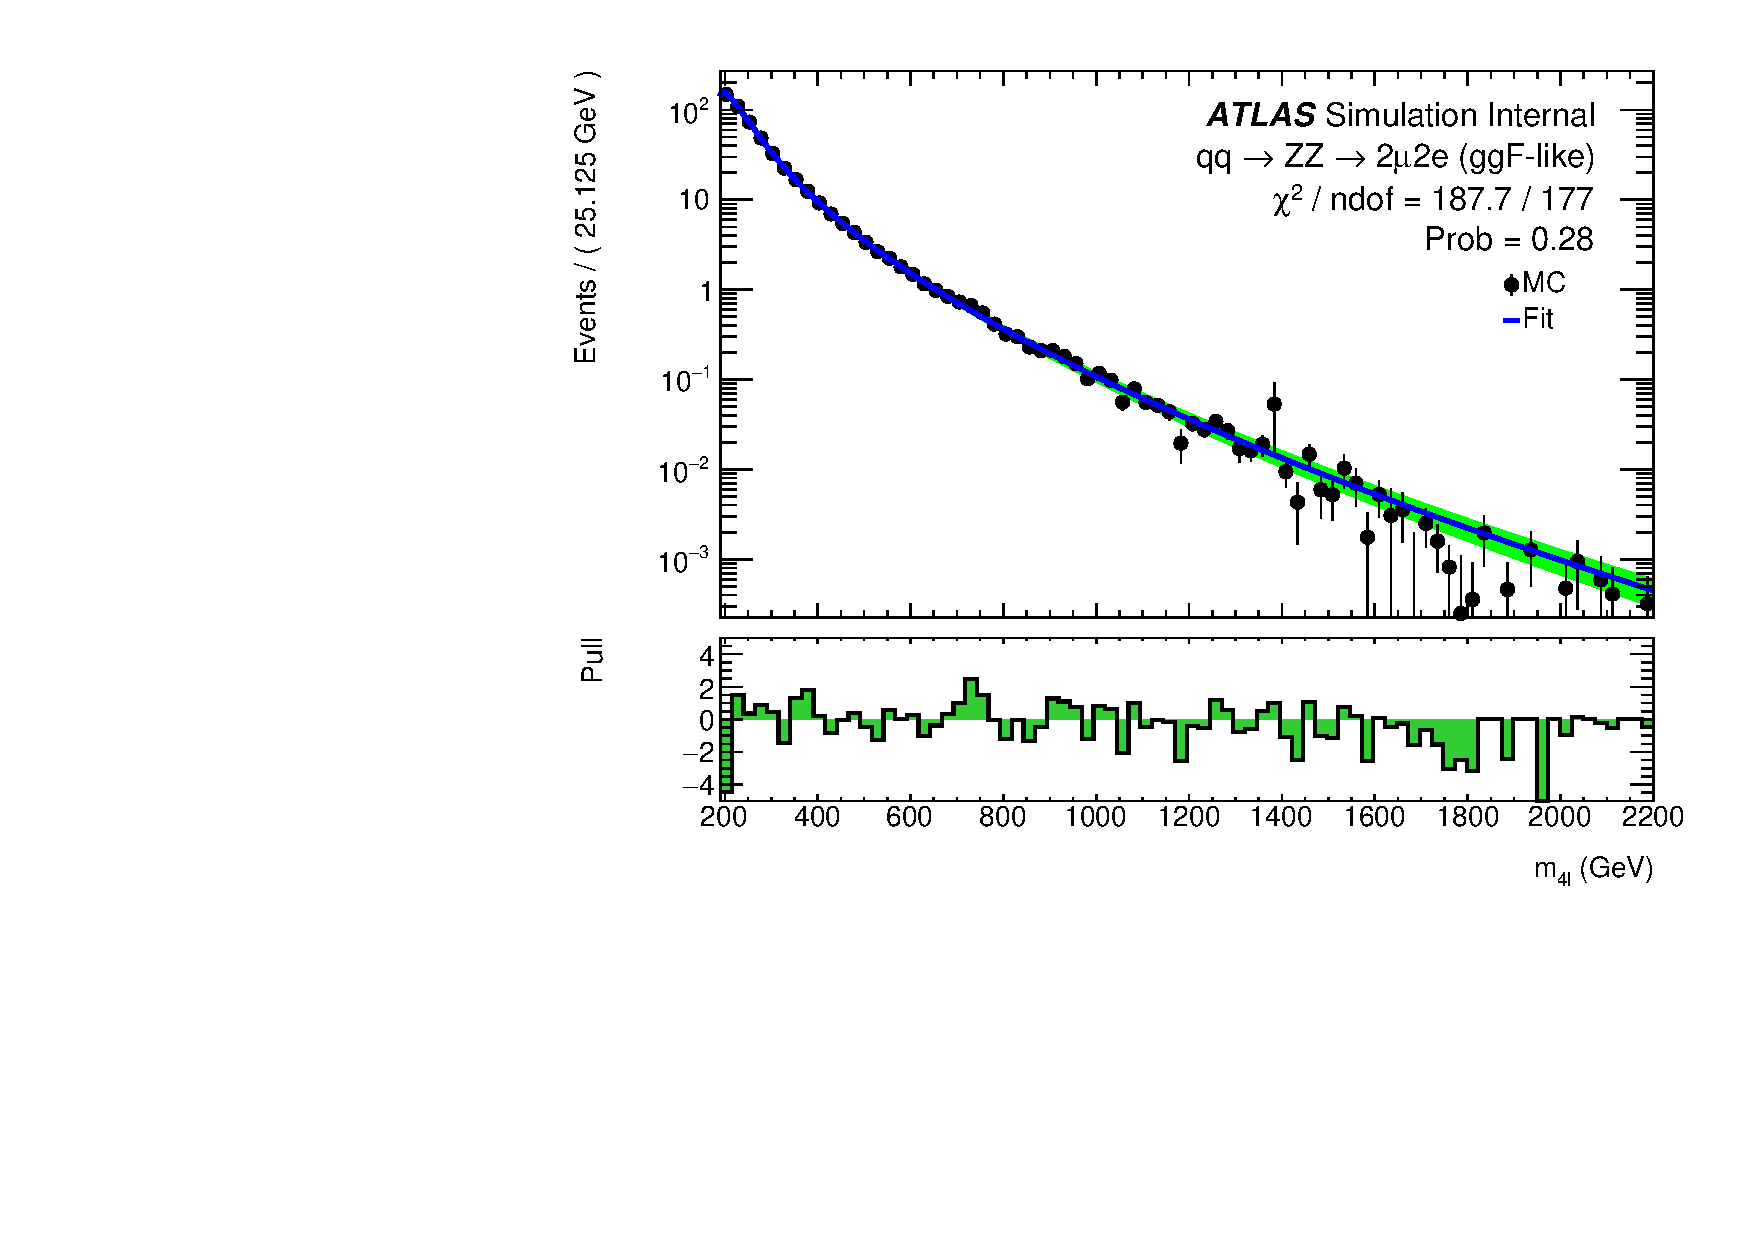
\includegraphics[width=0.32\textwidth]{figures/HMHZZ/background/dnn/bkg_shape_qqZZ_ggF_2mu2e_190_to_2200_log.pdf} \\
    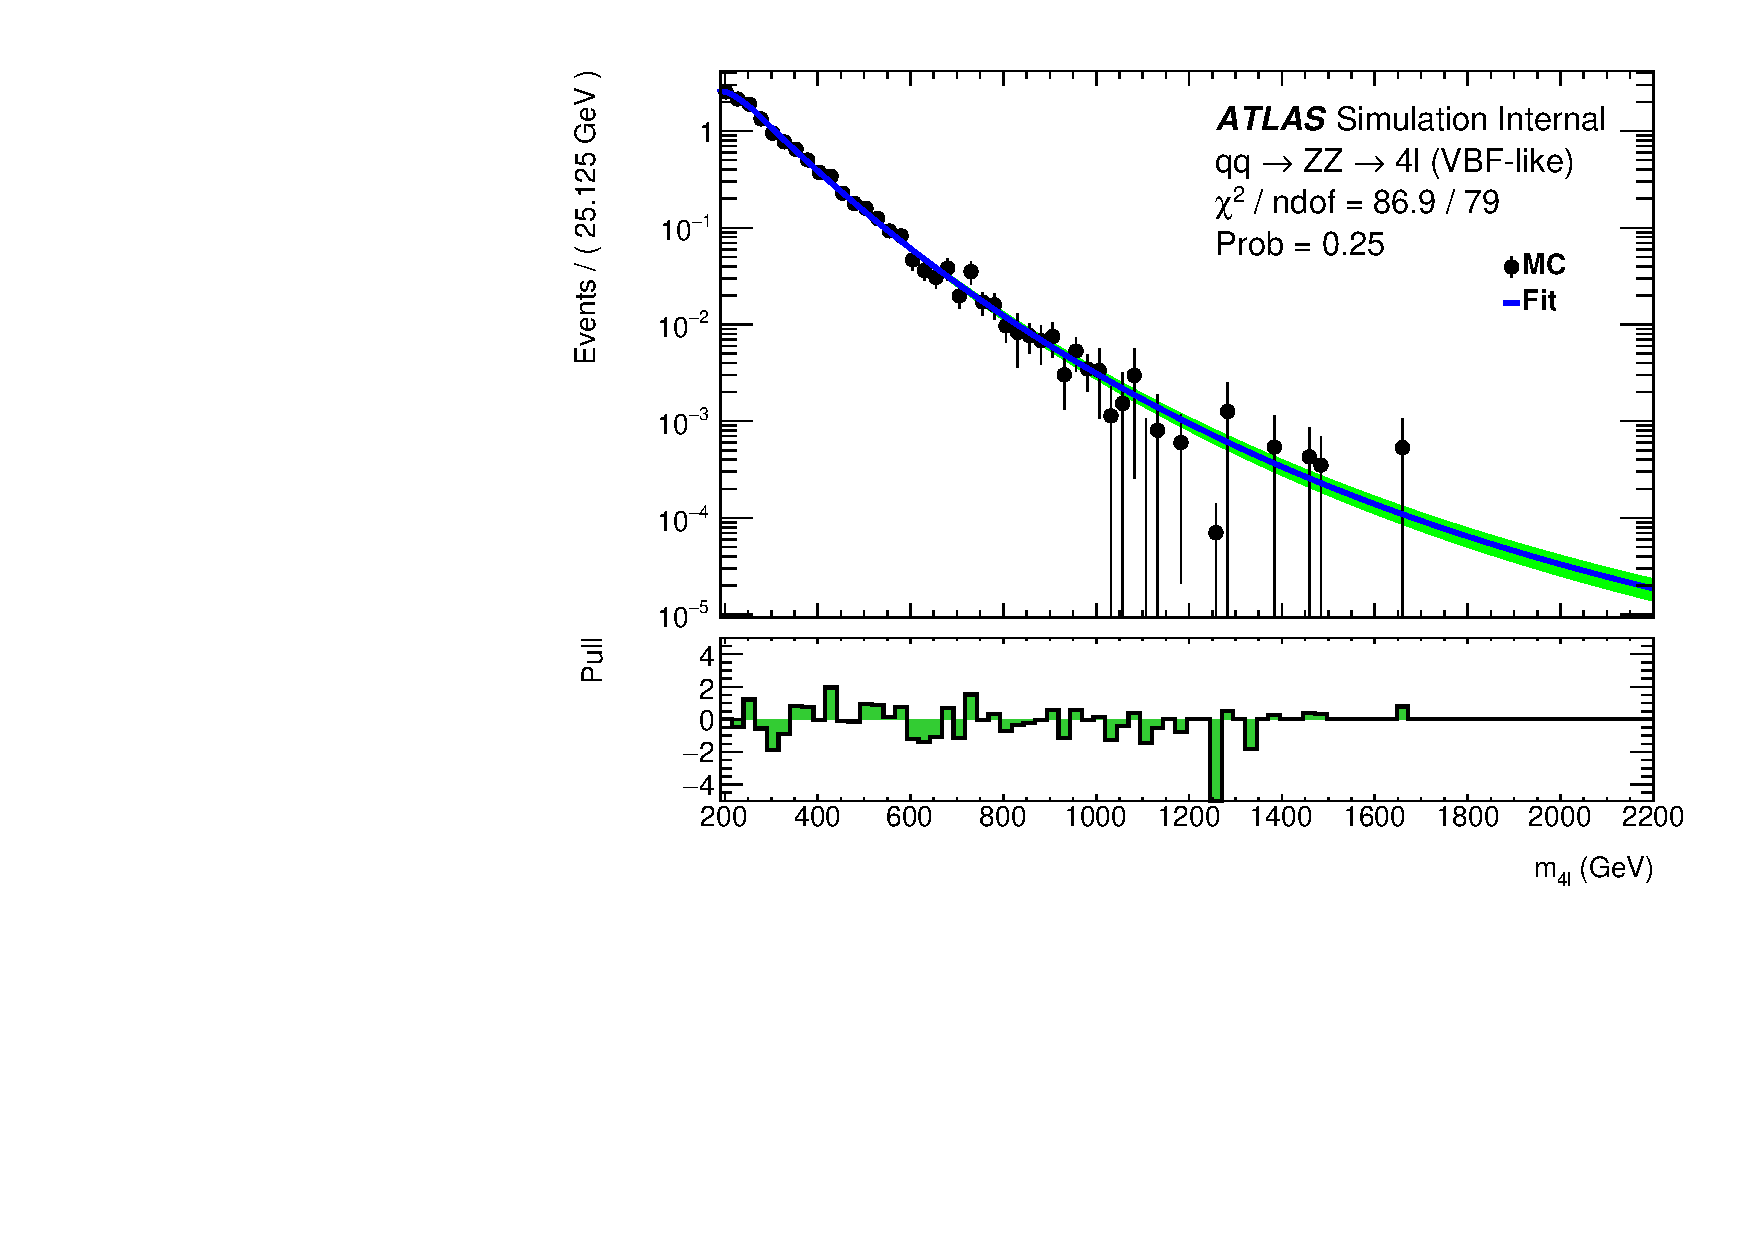
\includegraphics[width=0.32\textwidth]{figures/HMHZZ/background/dnn/bkg_shape_qqZZ_VBF_incl_190_to_2200_log.pdf}
    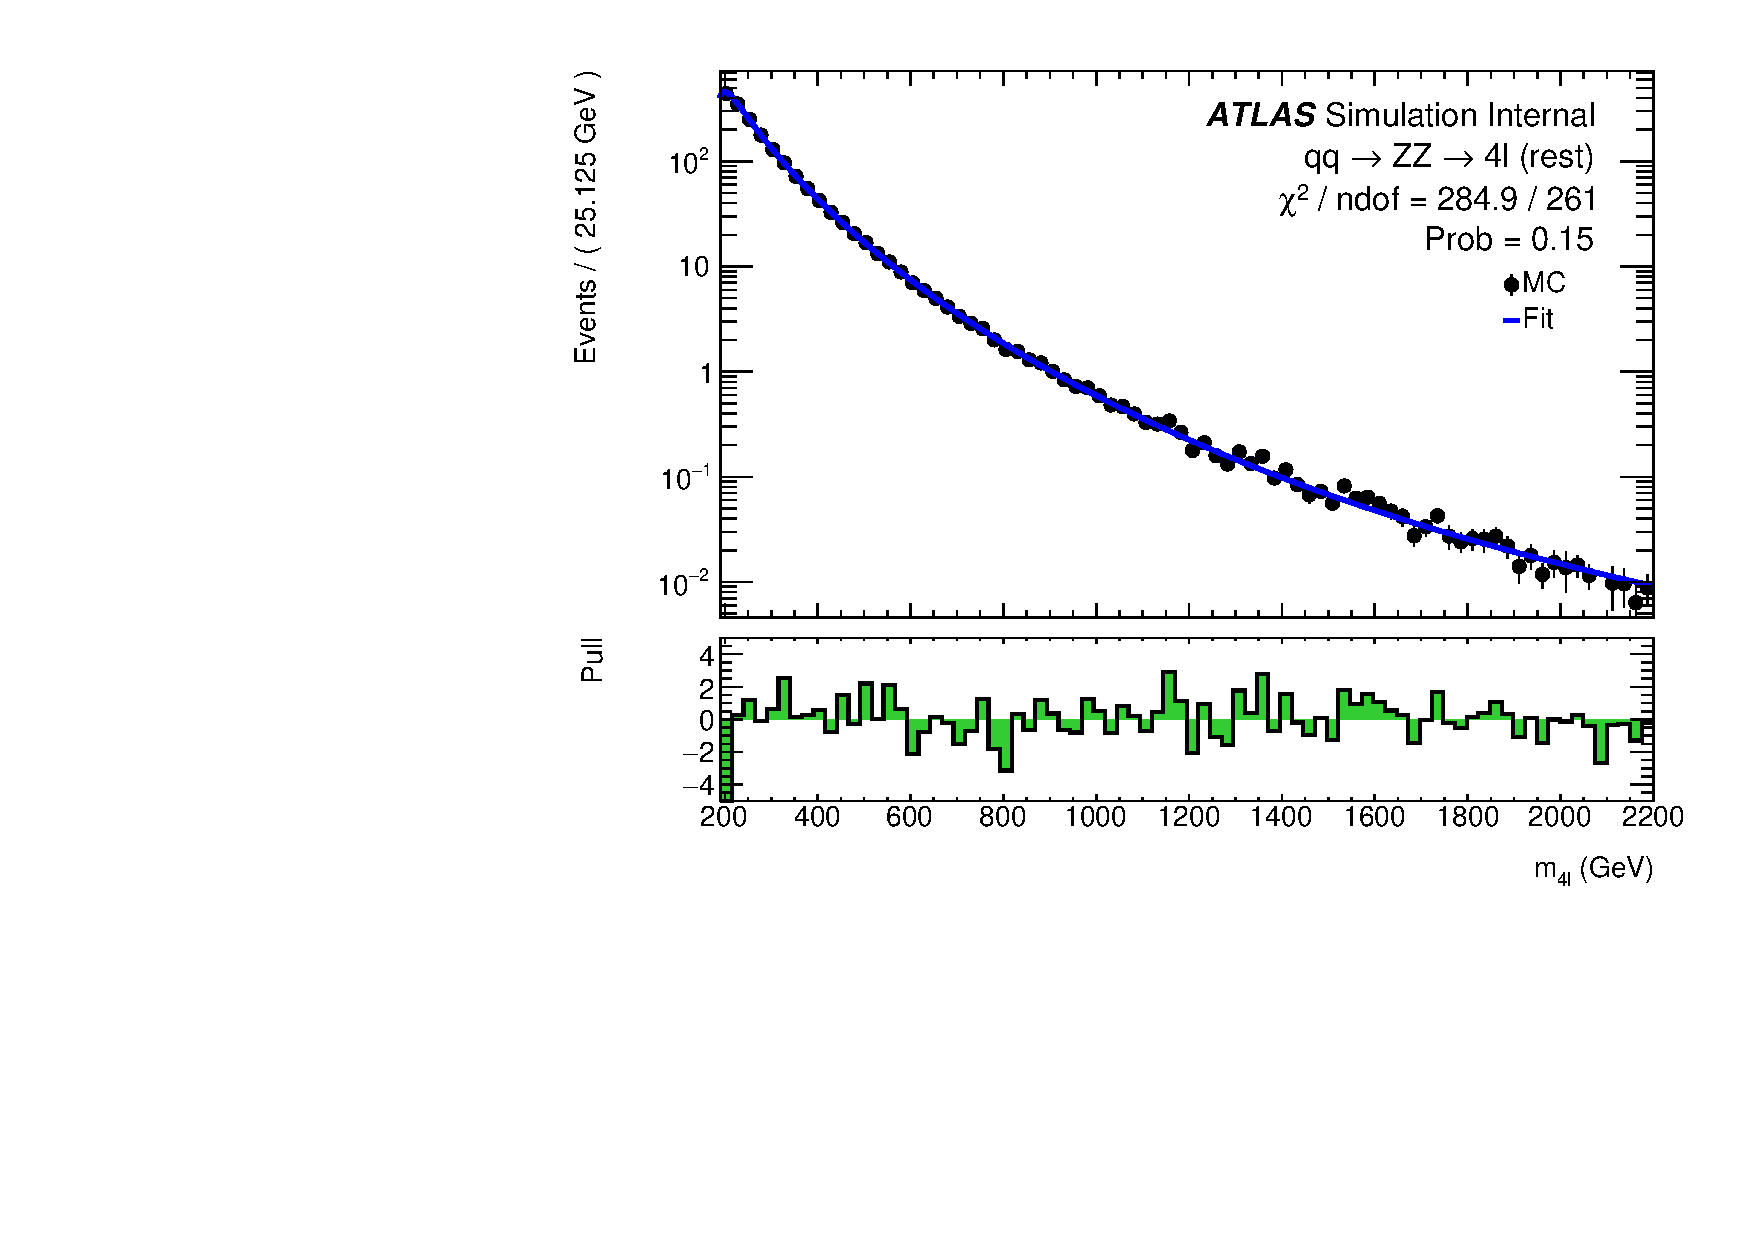
\includegraphics[width=0.32\textwidth]{figures/HMHZZ/background/dnn/bkg_shape_qqZZ_rest_190_to_2200_log.pdf}
    \caption{Distributions of the \mfl invariant mass fit projections of the \qqZZ background samples for the $4\mu$,
    $4e$ and $2\mu 2e$ final states in the ggF-MVA-high category, the $4\ell$ inclusive ggF-MVA-low category and VBF-MVA-enriched category.
    DNN-based categorization is used.} 
    \label{fig:qqZZ_m4l_shape_all_DNN}
\end{figure}

\begin{figure}[htbp]
    \centering
    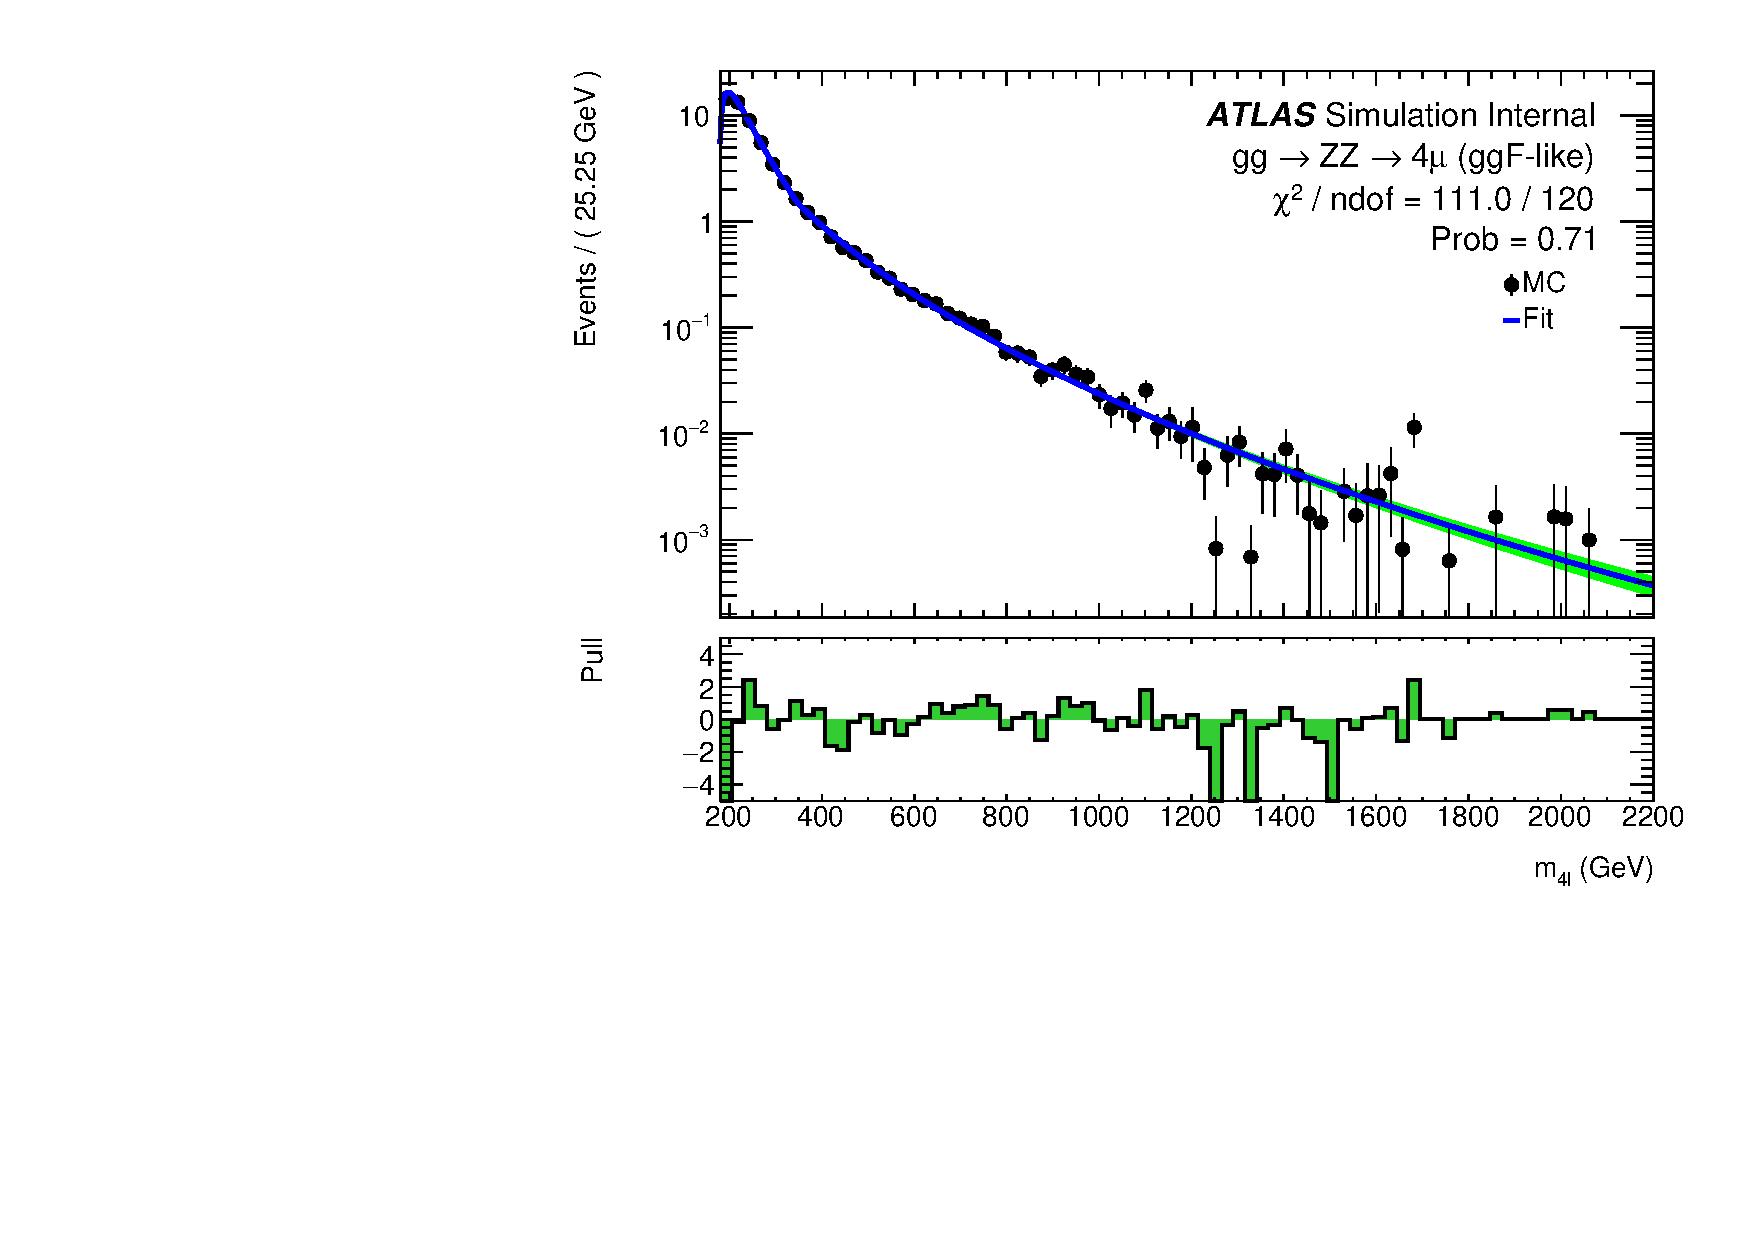
\includegraphics[width=0.32\textwidth]{figures/HMHZZ/background/dnn/bkg_shape_ggZZ_ggF_4mu_180_to_2200_log.pdf}
    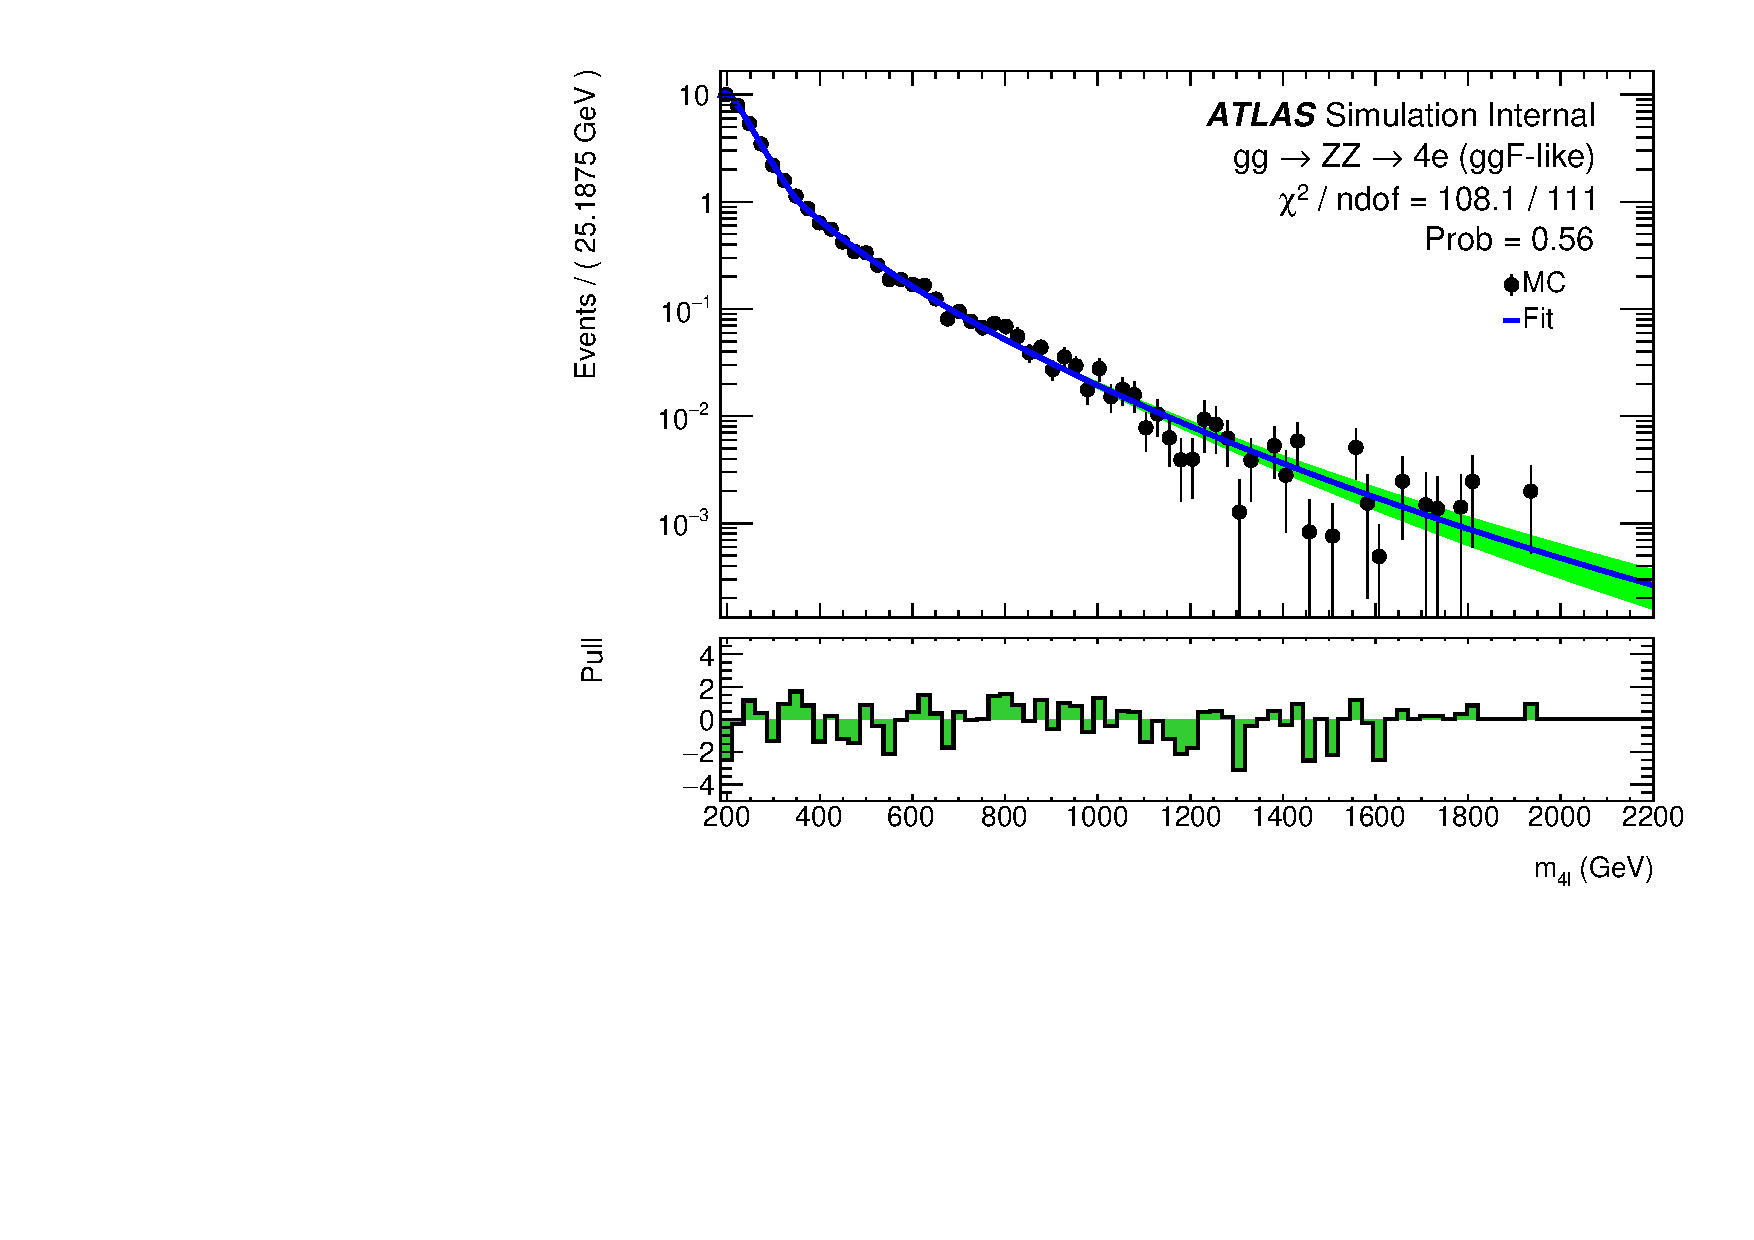
\includegraphics[width=0.32\textwidth]{figures/HMHZZ/background/dnn/bkg_shape_ggZZ_ggF_4e_185_to_2200_log.pdf}
    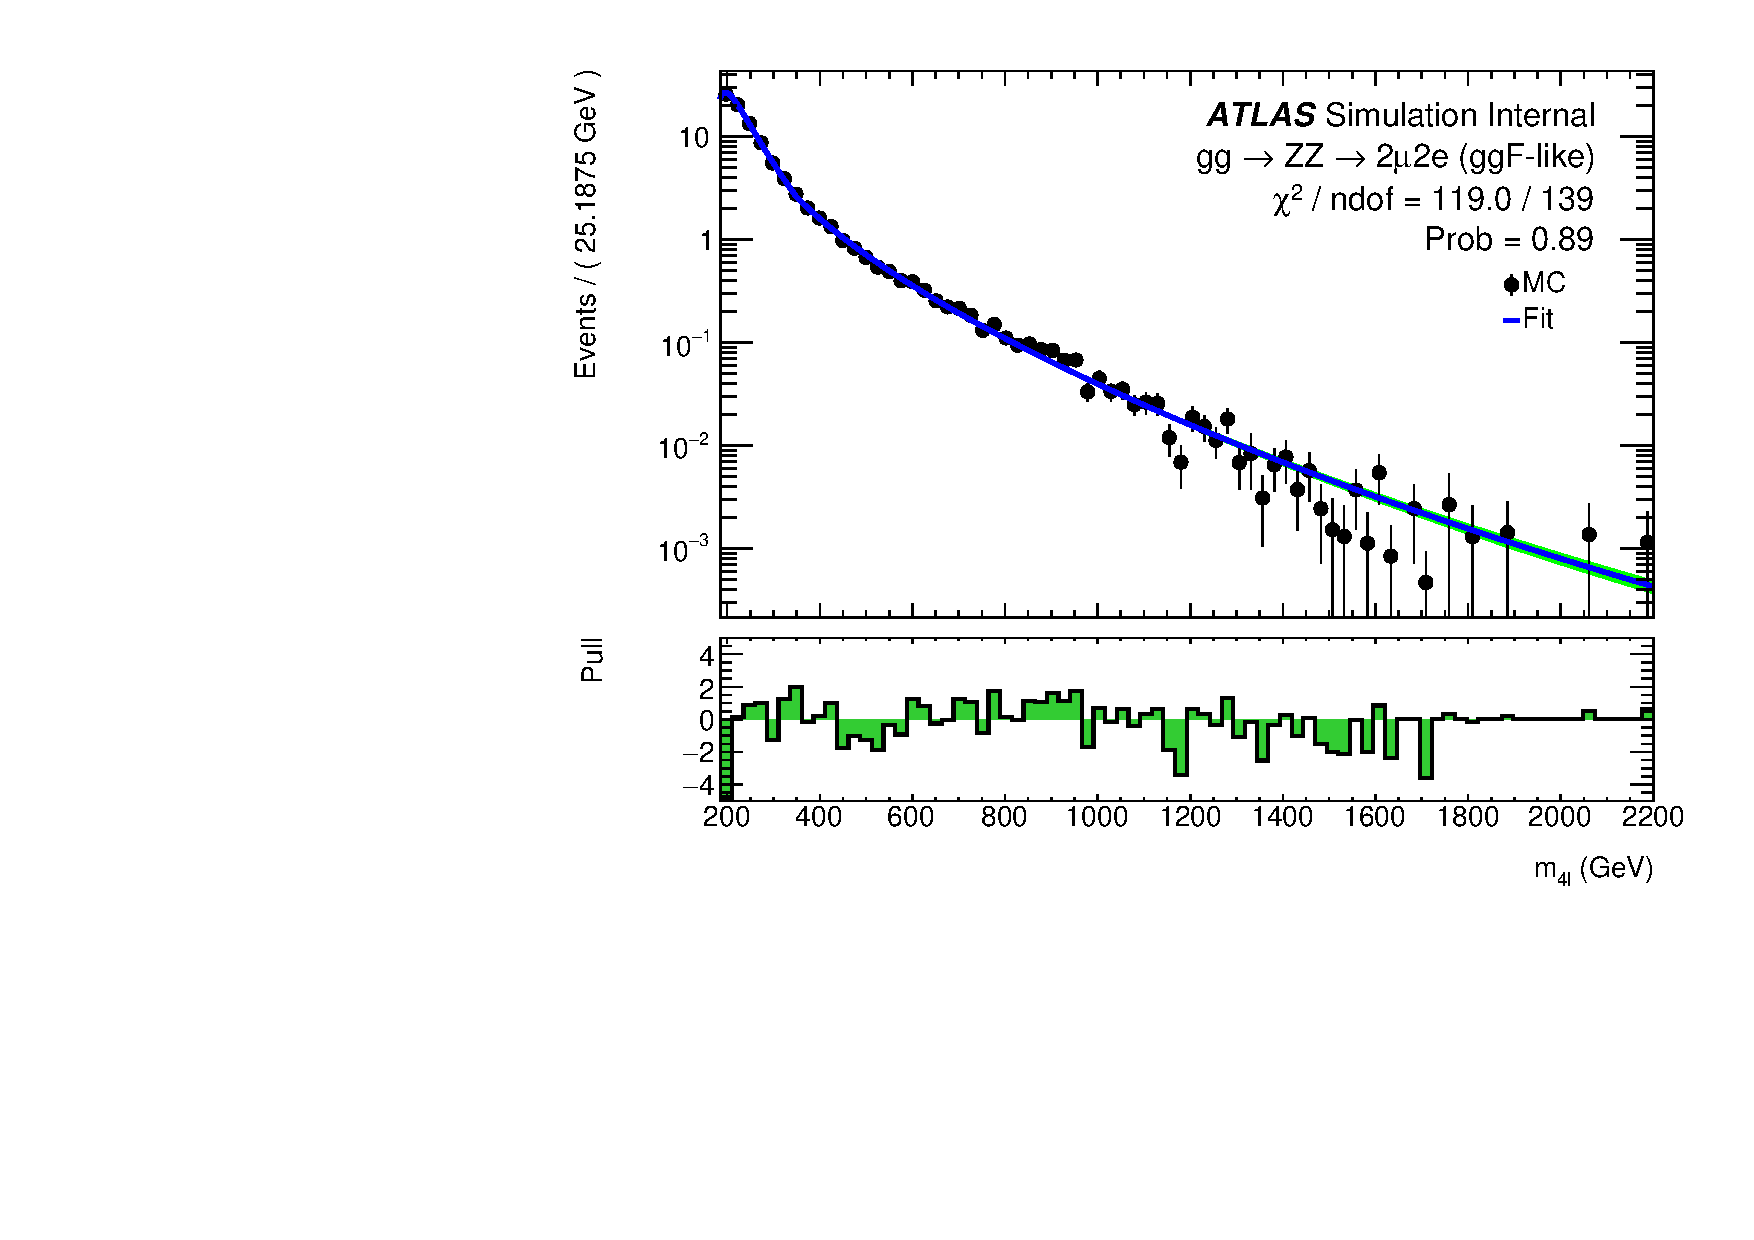
\includegraphics[width=0.32\textwidth]{figures/HMHZZ/background/dnn/bkg_shape_ggZZ_ggF_2mu2e_185_to_2200_log.pdf} \\
    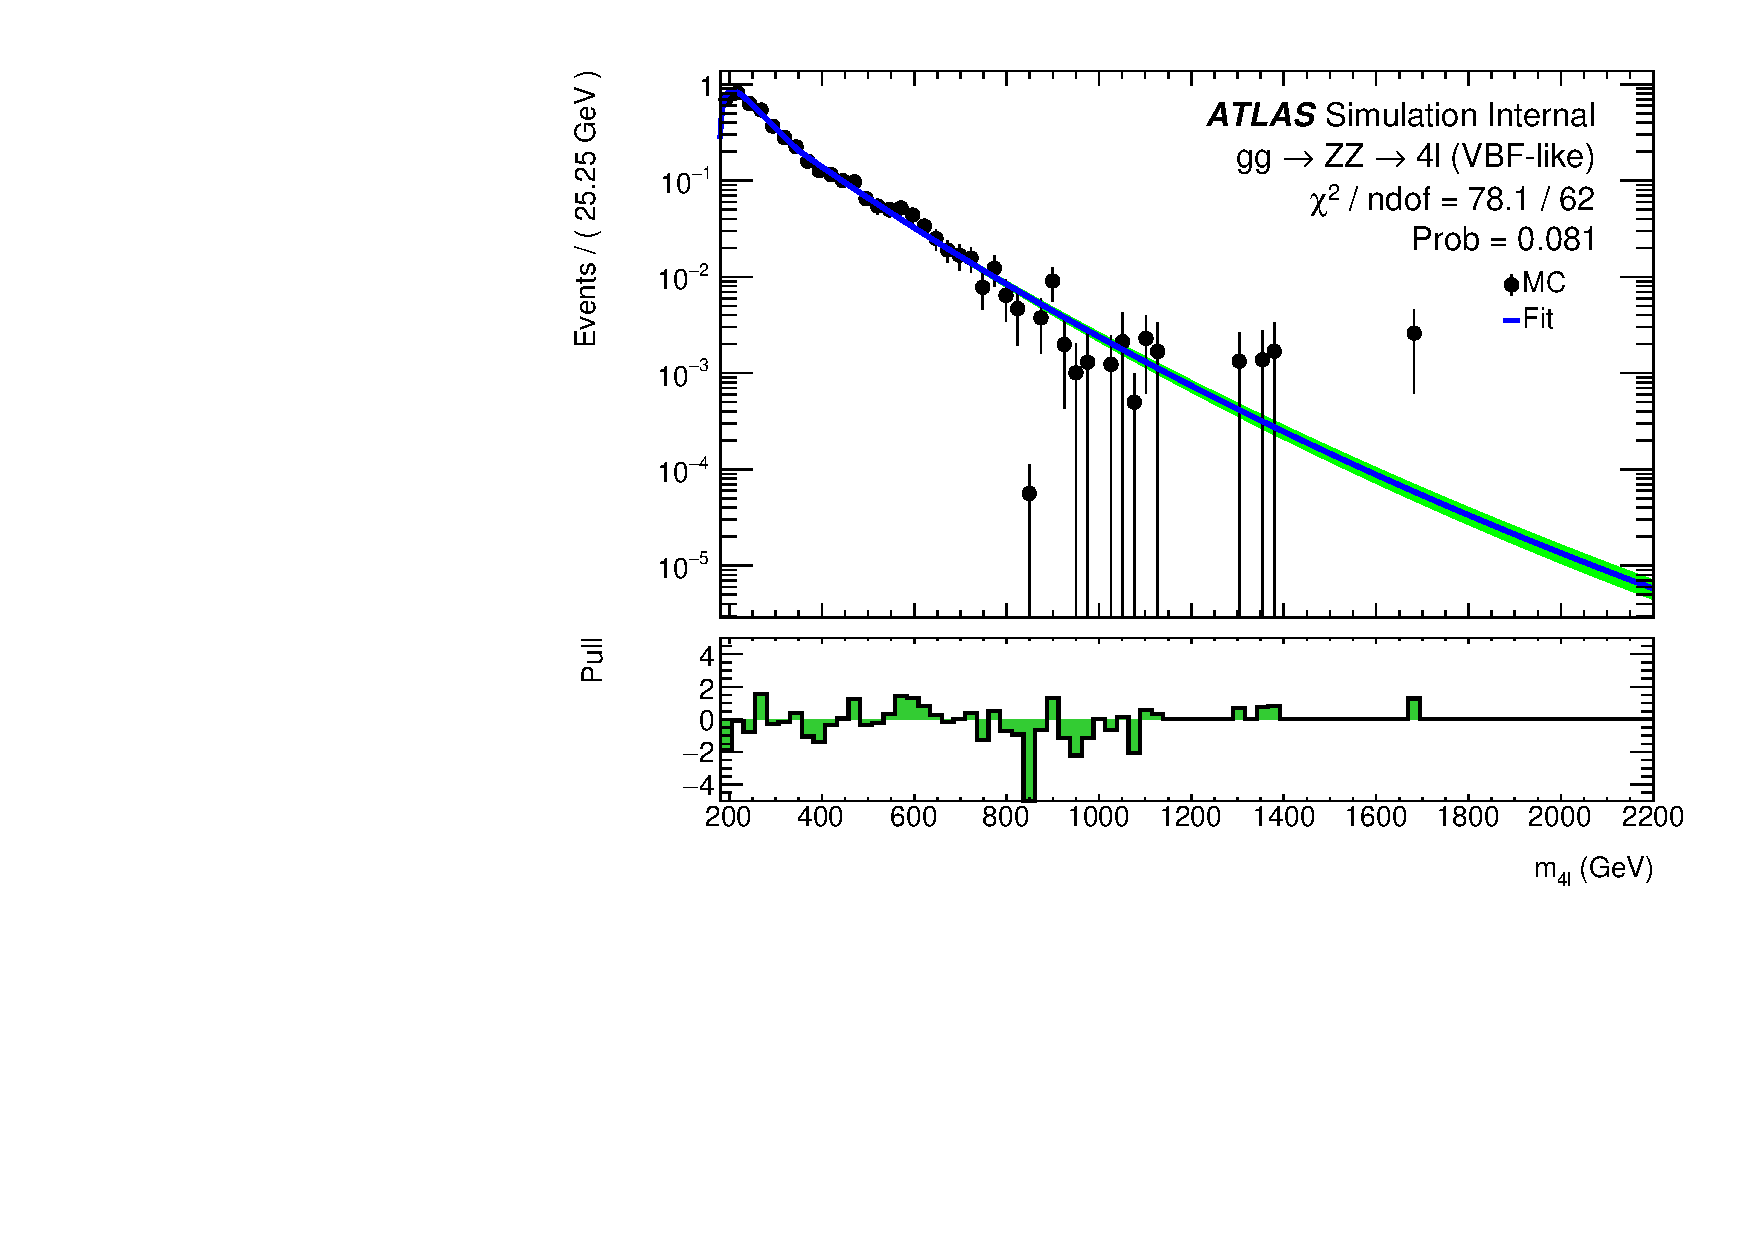
\includegraphics[width=0.32\textwidth]{figures/HMHZZ/background/dnn/bkg_shape_ggZZ_VBF_incl_180_to_2200_log.pdf}
    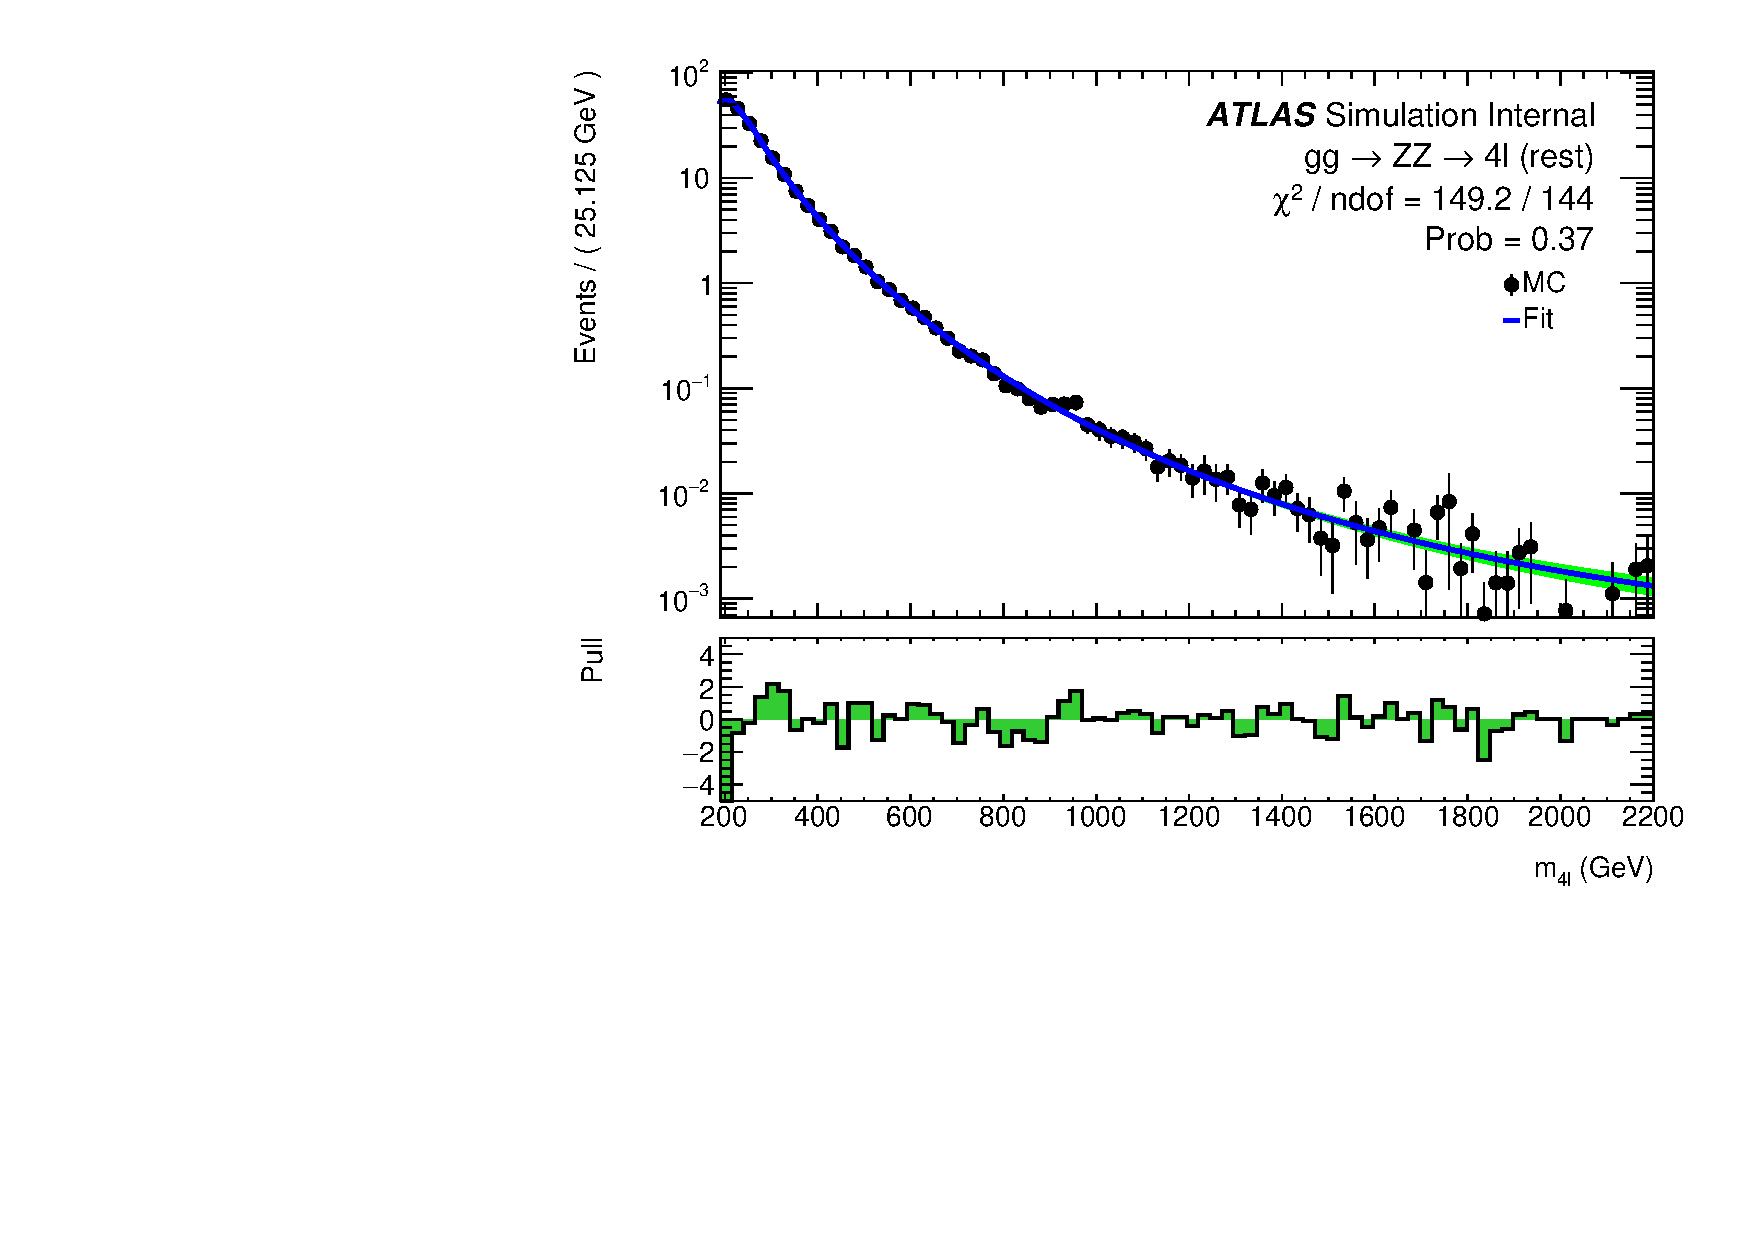
\includegraphics[width=0.32\textwidth]{figures/HMHZZ/background/dnn/bkg_shape_ggZZ_rest_190_to_2200_log.pdf}
    \caption{Distributions of the \mfl invariant mass fit projections of the \ggZZ background samples for the $4\mu$,
    $4e$ and $2\mu 2e$ final states in the ggF-MVA-high category, the $4\ell$ inclusive ggF-MVA-low category and VBF-MVA-enriched category.
    DNN-based categorization is used.} 
    \label{fig:ggZZ_m4l_shape_all_DNN}
\end{figure}

\begin{figure}[htbp]
    \centering
    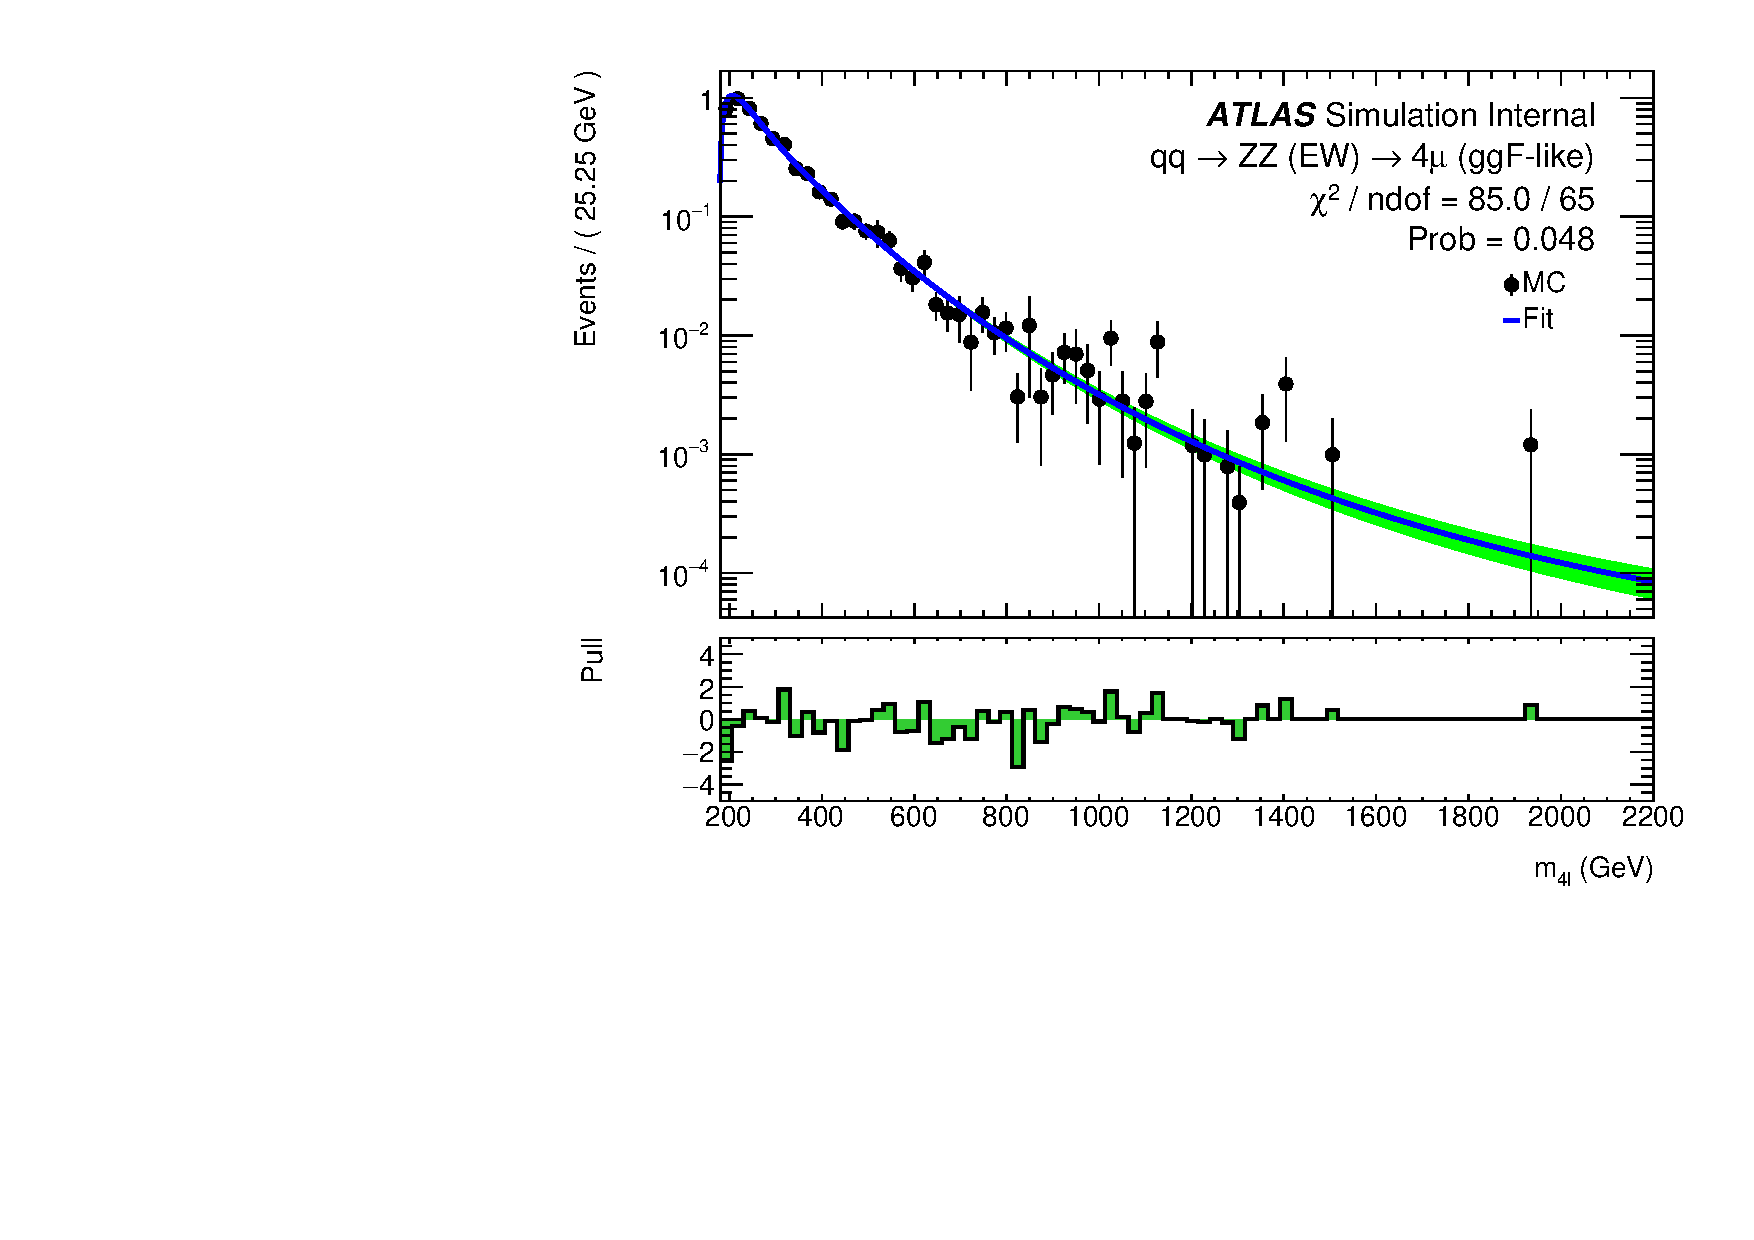
\includegraphics[width=0.32\textwidth]{figures/HMHZZ/background/dnn/bkg_shape_qqZZEW_ggF_4mu_180_to_2200_log.pdf}
    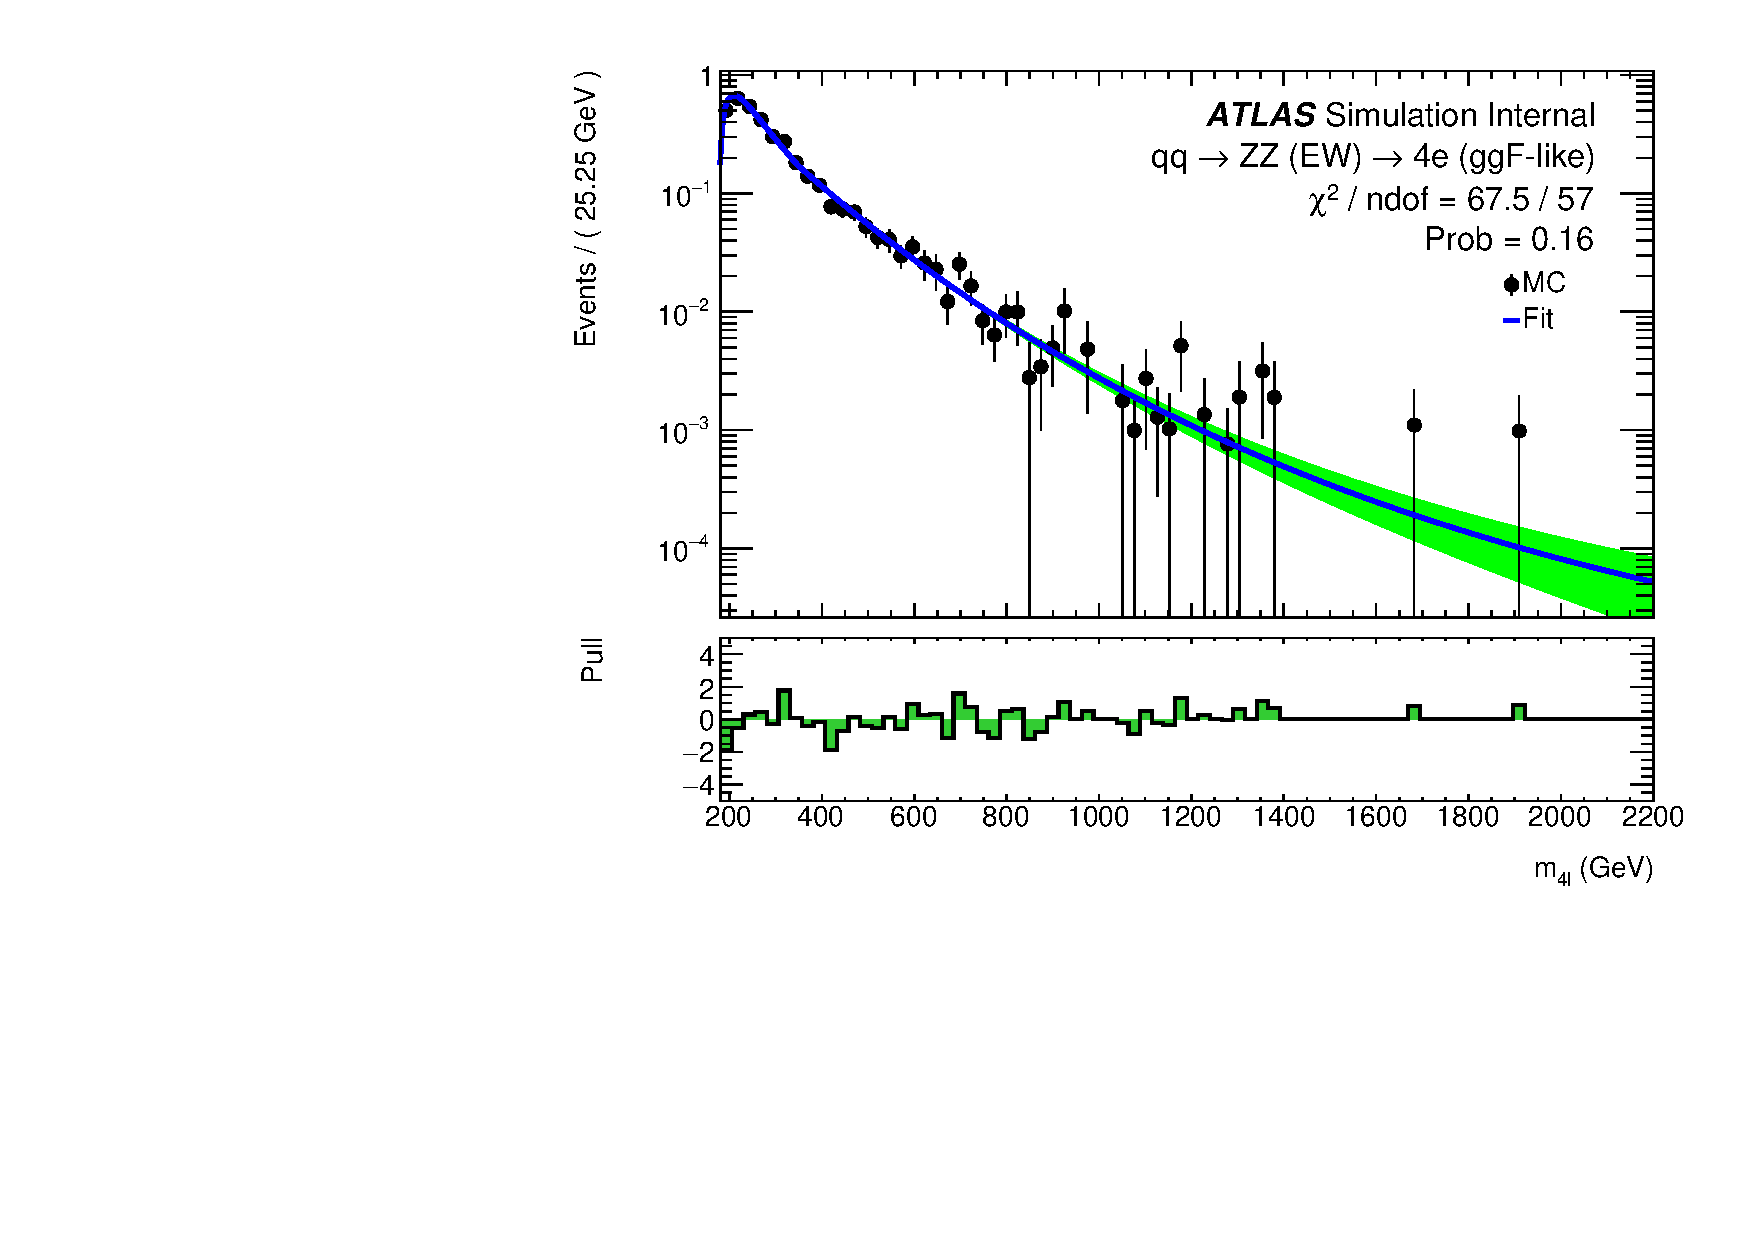
\includegraphics[width=0.32\textwidth]{figures/HMHZZ/background/dnn/bkg_shape_qqZZEW_ggF_4e_180_to_2200_log.pdf}
    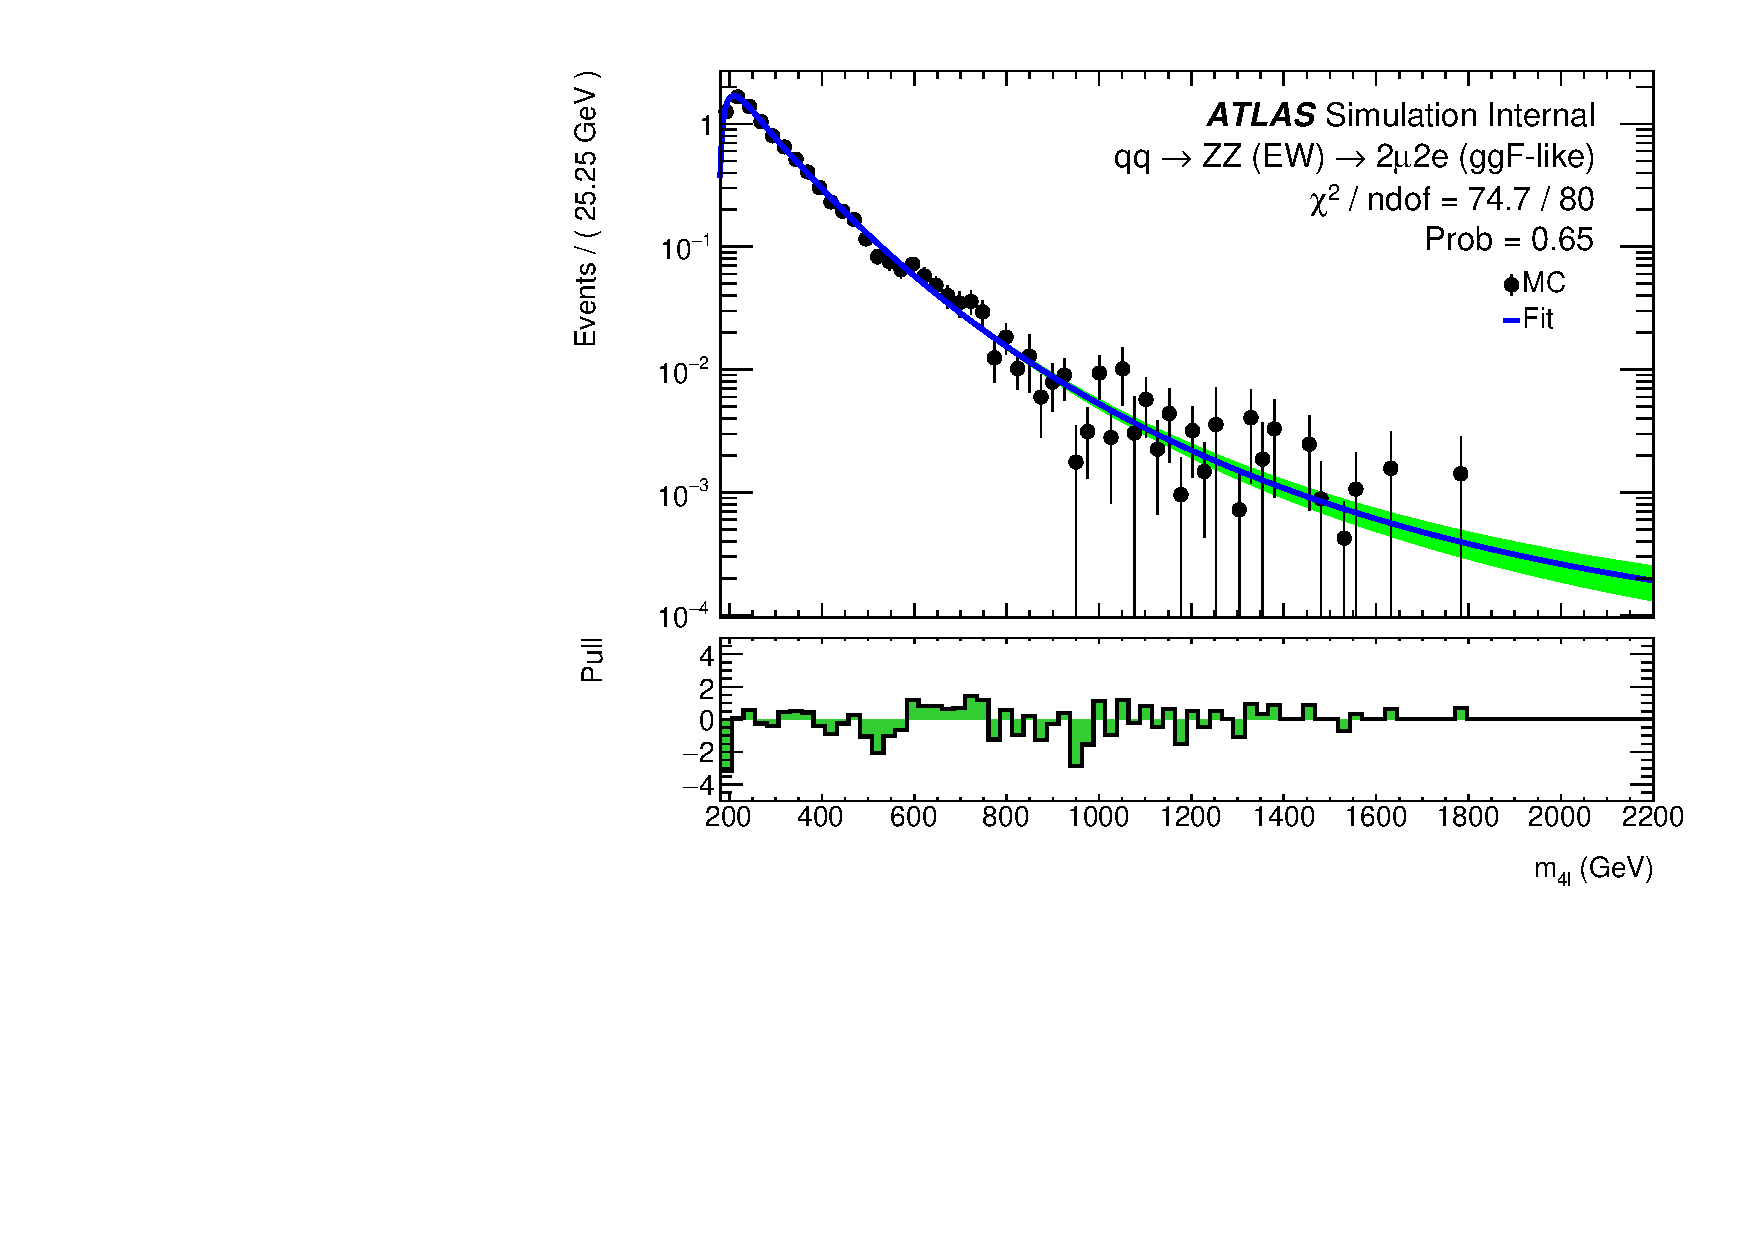
\includegraphics[width=0.32\textwidth]{figures/HMHZZ/background/dnn/bkg_shape_qqZZEW_ggF_2mu2e_180_to_2200_log.pdf} \\
    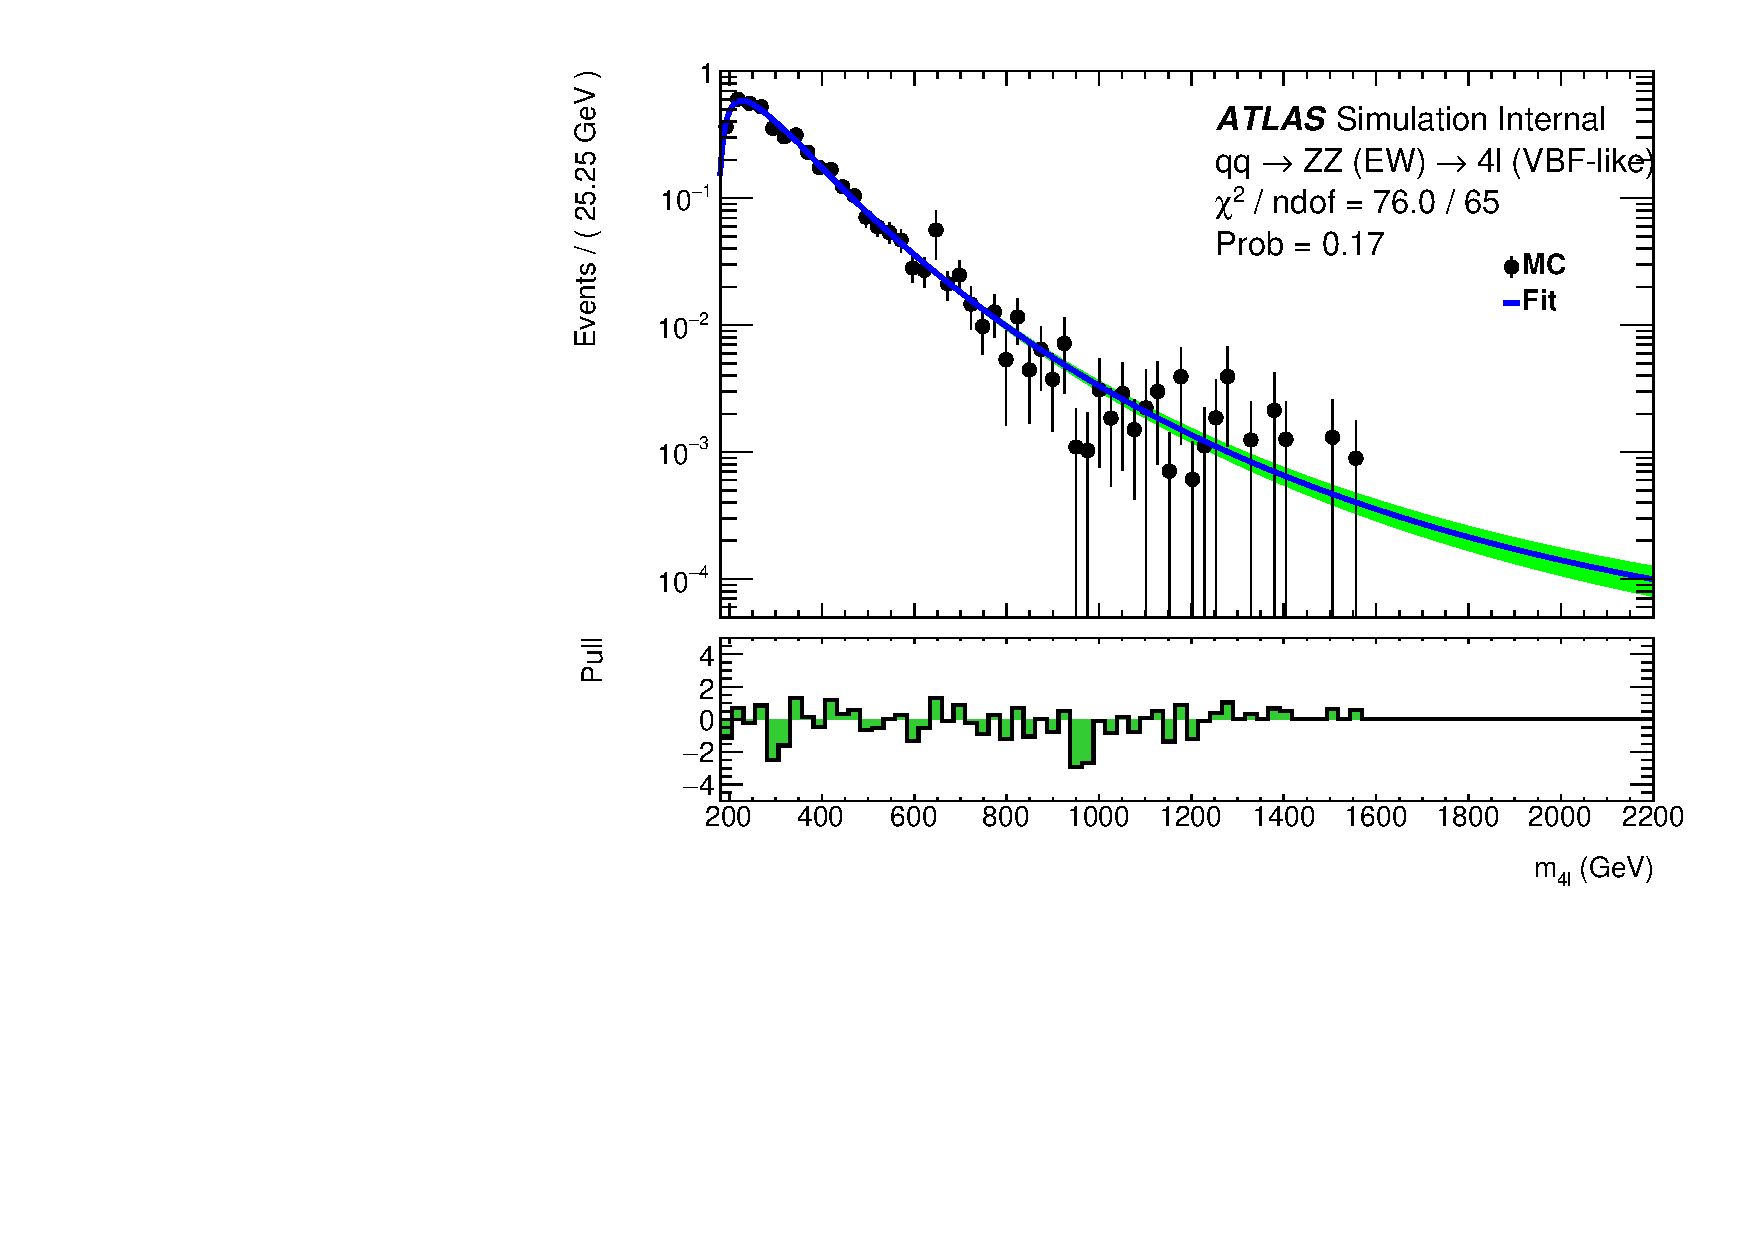
\includegraphics[width=0.32\textwidth]{figures/HMHZZ/background/dnn/bkg_shape_qqZZEW_VBF_incl_180_to_2200_log.pdf}
    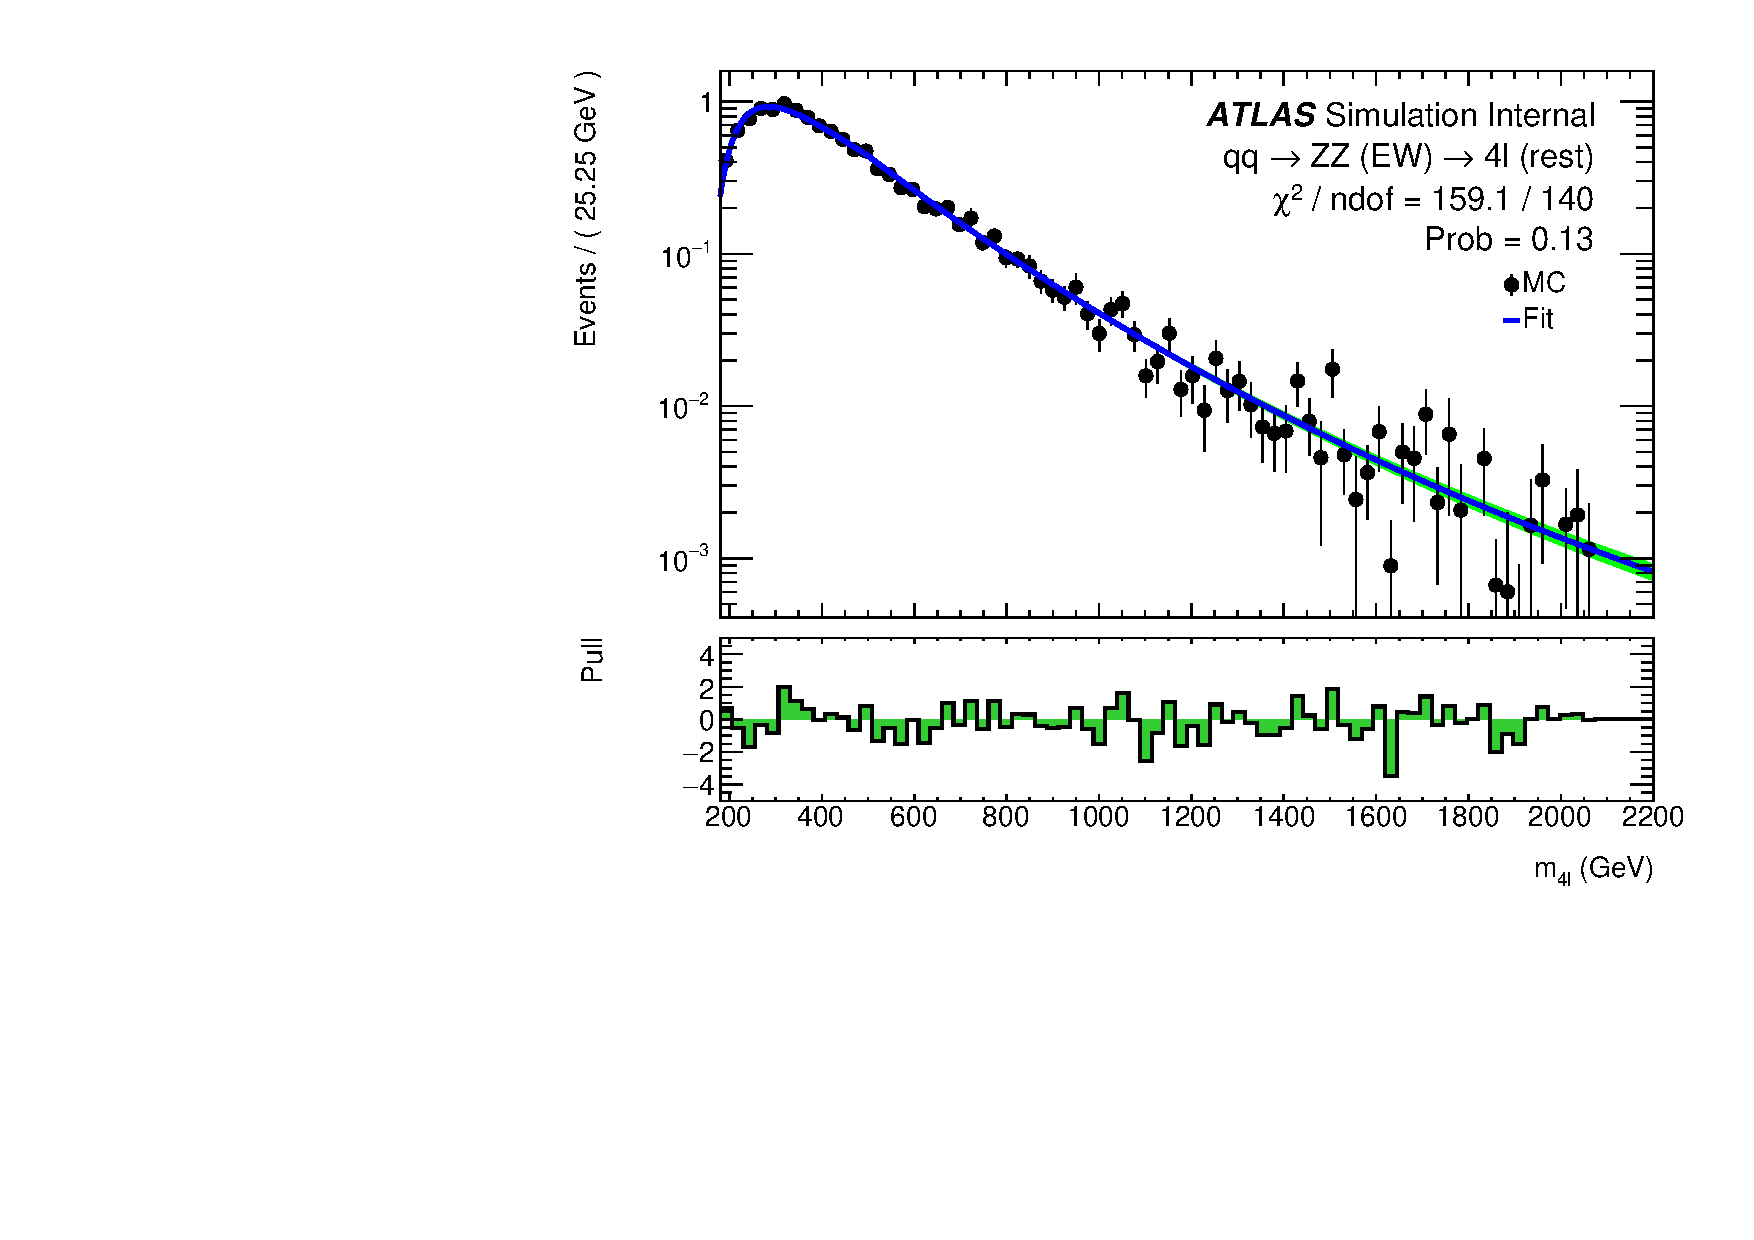
\includegraphics[width=0.32\textwidth]{figures/HMHZZ/background/dnn/bkg_shape_qqZZEW_rest_180_to_2200_log.pdf}
    \caption{Distributions of the \mfl invariant mass fit projections of the \qqZZ (EW) background samples for the
    $4\mu$, $4e$ and $2\mu 2e$ final states in the ggF-MVA-high category, the $4\ell$ inclusive ggF-MVA-low category and VBF-MVA-enriched category.
    DNN-based categorization is used.} 
    \label{fig:qqZZEW_m4l_shape_all_DNN}
\end{figure}

\subsection{Reducible backgrounds}

Similar as section~\ref{sec:background}, the reducible backgrounds include \Zjet (consists of both heavy- and light-flavour jets), top quark pair, and $WZ$ production, which contain fake and non-isolated leptons.
The simulations are not very robust in terms of the selection efficiencies.
Thus, the data-driven method is applied to estimated the normalization of those processes in different control regions (CRs).
The estimations in this analysis are performed separately for \llmumu and \llee final states, with slightly different approaches for ``muon'' and ``electron'' backgrounds.

The ``electron'' backgrounds mostly come from process of a $Z$ boson with light-flavour jets ($Z$+LF) misidentified as electrons.
The large contribution of ``muon'' backgrounds come from heavy-flavour jets produced in association with a $Z$ boson ($Z$+HF) or in the decays of top quark.
The estimations are done following the common H4l studies without a specific \mfl range requirement~\cite{PhysRevD.91.012006}, and then the corresponding fraction of event yield in $\mfl > 200~\gev$ is calculated from MC simulation.

\textbf{\llmumu final states} 

The normalizations of ``muon'' backgrounds are extracted from simultaneous fits of the leading lepton pair's invariant mass ($m_{12}$) in four orthogonal CRs:
\begin{itemize}
	\item \textbf{Inverted $d_{0}$ CR}: this CR is formed by inverting the $d_{0}$ selection for at least one lepton in subleading lepton pair while the leptons in leading pair are required to pass all standard selection.
This CR enhances $Z$+HF and \ttbar as leptons from heavy-flavour hadronic decays are characterised by large d0.
	\item \textbf{$e\mu+\mu\mu$ CR}: this CR is formed using an opposite-charge different-flavour dilepton in leading pair.
It aims to enhance \ttbar background as the leading lepton pair cannot come from $Z$ boson decay.
	\item \textbf{Inverted isolation CR}: in this CR, leptons in leading pair are required to satisfy all standard analysis selection, while for leptons in subleading pair, they are required to pass $d_{0}$ selection but have at least one of them failing isolation selection.
This CR enhances the events from $Z$+LF processes while suppress $Z$+HF by $d_{0}$ cut.
	\item \textbf{Same-sign CR}: in this CR, the leptons in subleading pair are required to have same-charge, while the leading pair still passes standard selection.
This CR is not dominant by any specific background since all reducible backgrounds could have sizable contribution in it.
\end{itemize}

The fit results of normalizations are then propagated to signal region (SR) by applying transfer factors to account the difference of selection efficiencies between SR and CRs.
The transfer factors are computed using $Z+\mu$ MC samples.

\textbf{\llee final states} 

The ``electron'' backgrounds are estimated in $3\ell+X$ CR, where $X$ denotes the lower \pt electron in the subleading pair.
The selection and identification criterias for $X$ are relaxed , while other three leptons must satisfy the standard selection.
In this case, $X$ could be a light-flavour jet, a photon conversion or an electron from heavy-flavour hadron decay.
Moreover, the subleading pair is required to have same charge dilepton to ensure the orthogonality to the signal region.
The normalization of backgrounds are obtained based on a fit to the number of hits in the innermost ID layer in CR,
and the transfer factors are computed from $Z+e$ simulated sample.

The \mfl shapes of reducible backgrounds are obtained from MC simulation in signal region, and then smoothed by an one-dimensional kernel estimation,
which models the input data as a superposition of Gaussian kernels, one for each data point with contributing $1/N$ to total integral $N$~\cite{Cranmer:2000du}.
The difference from using different smoothing strength ($\rho$) in kernel estimation is taken into account as additional shape uncertainties for these reducible backgrounds.
